%==================================================================================================
%   LUKES THESIS TEMPLATE 1.2
%   -------------------------
%   This template is based upon the offcial IMM PhD Thesis template, it is enhanced with a number
%   of new features and a number of errors have fixed. This template is intended to be complied to
%   PDF using PDFLATEX and is tested using the MiKTeX 2.9 LaTeX distribution.
%   It is based on the official DTU-IMM Thesis template by Finn Kuno Christensen in 2009.
%   Small bugfixes by Kasper Laursen in 2012 and 2013.
%   -------------------------
%   Last Updated: 2012-09-19
%   Contact: lthhe@imm.dtu.dk
%==================================================================================================
%
%==================================================================================================
% DOCUMENT SETUP
%==================================================================================================
\documentclass[10pt,twoside]{book}                  %Official DTU-IMM Thesis document setup
%
%Set to 'print' for printed version, use 'net' for online version
\def\thesisversion{print}
%
%==================================================================================================
% PACKAGES
%==================================================================================================
\usepackage[square, sort, comma, numbers]{natbib}	%needed for nice bibliography
\usepackage[nogin]{Sweave}	%needed to use R plots and tables
%\usepackage{float}
%\usepackage{booktabs}
\usepackage{colortbl}
\usepackage{rotating}	%needed to rotate the tables sideways
\usepackage{VladThesis}                             %Import Thesis base style
\usepackage{subfig}
\usepackage{algorithm,algpseudocode}
\usepackage{amstext}
\usepackage{tikz}
\usetikzlibrary{arrows,decorations.pathmorphing,fit,positioning}

\newcommand{\dir}{\text{Dirichlet}}
\newcommand{\mult}{\text{Multinomial}}
\newfloat{algorithm}{t}{lop}

%input{PhDMacros}                                   %Thesis specific macros
%
%==================================================================================================
% THESIS PROPERTIES (Modifiy these fields with your details)
%==================================================================================================
\def\thesisauthor{Vlad Octavian Sandulescu}                     %Author
\def\thesistitle{Opinion spam detection through semantic similarity}               %Title 
\def\thesishandin{21-May}                       %Submission date (Day-Month}
\def\thesisdegree{M.Sc.}                              %Degree ('B.Eng', 'B.Sc.', 'M.Sc.' or 'PhD')
\def\thesisyear{2014}                               %Submission year
\def\thesisnumber                             %DTU-IMM Serial number (do not include year)
\def\thesisISSN{0000-0000}                          %ISSN number
\def\thesiskeywords{Keywords are, comma separated}  %PDF keywords
\derivethesisprops                                  %Derive dependent properties
%
%==================================================================================================
% SECTION NUMBERING SETUP
%==================================================================================================
\setcounter{tocdepth}{2}                            %2 adds sections up to subsections
\setcounter{secnumdepth}{3}                         %Subsubsections get a number when this is 3
%
%==================================================================================================
% THESIS STRUCTURE  (Modifiy to include more chapters etc)
%==================================================================================================
\begin{document}
%------------------------
%Pre-frontmatter material
%------------------------
\prefrontmatter
%--------------------
%Frontmatter material
%--------------------
\frontmatter
\pagenumbering{roman}                               %Set frontmatter numbering style
\chapter{Summary}

In this thesis I study the problem of detecting fake reviews written by the same users under different identities and aim to use semantic similarity metrics to compute the relatedness between user reviews. This represents a new approach to opinion spam detection, meant to capture more information than a simple text similarity measure, such as the cosine similarity and tap deeper into the textual particularities of a review. It is aimed at spammers which use multiple anonymous profiles to post reviews by reusing previous text they had also written, replacing the main aspect words with synonyms, while still keeping the overall sentiment the same. 

There is one obvious but important assumption - the imagination of a spammer, like any human is limited and thus will not be able to write completely different reviews about an imaginary experience every single time. Thus, it is very likely he will partially reuse some of the content and aspects between reviews.

This thesis proposes a complete solution to detect opinion spam of one-time reviewers using semantic similarity. It also proposes a method to detect opinion spam using recent research models aimed at extracting product aspects from short texts, based on topic modeling and in particular on Latent Dirichlet Allocation. Another goal was to test this hypothesis on real-life reviews and make a comparison with the existing cosine-based vectorial similarity models.

This research also proposes to use density-based clustering to group reviews using simple behavioral features, proven to be linked to suspicious user activity. Clustering divides the reviews into smaller chunks, thus the number of comparisons is reduced considerably. The novelty of the topic modeling method is to use the similarity of the underlying topic distributions of the reviews to classify them as truthful or deceptive. 

Experimental results showed that semantic similarity can outperform the vectorial model in detecting deceptive reviews, capturing even more subtle textual clues. The precision score of the review classifier showed high results, enough to make the method viable to be integrated into a production detection system. The results of the topic modeling method showed that combining opinion spam detection with topic modeling may offer, for some number of topics, results in the vicinity of the semantic similarity models.                                   %English summary of Thesis
\markboth{}{}                                       %Set headings (left)(right)
%\input{SummaryDK}                                   %Danish summary of Thesis
%\markboth{}{}                                       %Set headings (left)(right)
\chapter{Preface}

This thesis was prepared at the department of Informatics and Mathematical Modeling at the Technical University of Denmark in fulfillment of the requirements for acquiring a M.Sc. in Computer Science and Engineering.

The thesis deals with the problem of opinion spam - deceptive reviews posted on review websites by dishonest users trying to promote or demote certain products and sellers.

The thesis consists of an introduction to the problem of opinion spam and the current state-of-the-art research models that deal with it. The following chapters propose, describe and discuss the methods used to design a complete solution to detect opinion spam using semantic similarity, as well as a detection method based on recent research models aimed at extracting product aspects from short texts, using topic modeling and in particular Latent Dirichlet Allocation.

%==================================================================================================
% SIGNATURE AREA
%==================================================================================================
\vspace{20mm}
\begin{center}
    \hspace{20mm} Lyngby, \thesishandin-\thesisyear
    \vspace{10mm}
    \newline
  %Update signature image file in line below
%    \includegraphics[width=100mm,height=30mm,keepaspectratio]{figures/Signature}
    \thesisauthor
\end{center}
%\begin{flushright}
%    \thesisauthor
%\end{flushright}
% % % EOF % % %                                     %Preface
\markboth{}{}                                       %Set headings (left)(right)
\chapter{Acknowledgements}

I thank my supervisor Paul Pop for his support and guidance not only while writing this thesis, but also during several courses I took while being a student at Technical University of Denmark. 

I am grateful to my advisor Martin Ester, Professor at Simon Fraser University for his insightful advices during this last year. He has helped me narrow down my research problem and provided knowledgeable feedback step by step as I was developing the models.

I thank my colleagues Stine Mangor Tornmark and Jan Bülow at Trustpilot for granting my request to build and use a dataset for my research.


                            %Acknowledgements
\markboth{}{}                                       %Set headings (left)(right)
%------------------
% Table of contents
%------------------
\newpage\mbox{}\newpage
\chaptermark{Contents}
\pdfbookmark{\contentsname}{toc}
\renewcommand{\sectionmark}[1]{\markright{#1}}
\sectionmark{Contents}
\addtolength{\parskip}{-\baselineskip}
\tableofcontents
\addtolength{\parskip}{\baselineskip}
\renewcommand{\sectionmark}[1]{\markright{\thesection\ #1}}
%-------------
% Main content
%-------------
\mainmatter
\chapter{Introduction}\label{chapter:introduction}

Online reviews have become in recent years a very important resource for consumers when making purchases. The number of consumers that first read reviews about a product they wish to buy is constantly on the rise. Technology research company Gartner Inc. claims 31\% of consumers read online reviews before actually making a purchase \citet{Gartner2013}. As consumers increasingly rely on these ratings, the incentive for companies to try to produce fake reviews to boost sales is also increasing. Gartner predicts in 2014 as much as 15 percent of all social media reviews will consist of company paid fake reviews, \citet{Gartner2012}. Deceptive reviews have at least two major damaging effects for the consumers. First, they lead the consumer to make bad decisions when buying a product. After reading a bunch of reviews, it might look like a good choice to buy the product, since many users praise it. After, it turns out the product quality is way below expectations and the buyer is disappointed. Second, the consumer's trust in online reviews drops. 

Government regulations and exposure of fake reviews as well as of bad company practices should lead to an increase in the level of trust. Until the proper regulations will be enforced though across markets, some websites are trying to warn users about this practice and publish tips for people to spot fake reviews \citet{TheGuardian2013,Consumerist2010}. Large review websites have even resorted to public shaming to put pressure on businesses who tried to buy reviews to praise their brands. In 2012, Yelp ran its famous "sting" operation when the company displayed a consumer alert message on the profile pages of fraudulent companies. Although this strategy made many headlines, it was stopped after a short time, probably because it became obvious that competitors could actually hurt rival businesses by attempting to buy reviews in their name. 

Another major review website, TripAdvisor has been censured over their claim to offer “honest opinions from real travelers”, when the UK Advertising Standards Authority ruled that the statement was misleading to consumers and that non-genuine content could appear on the website. The company has been recently further shamed by a businessman who registered an imaginary restaurant and then wrote reviews for it. The hoax was detected by TripAdvisor after several months \citet{Forbes2013}.

\section{Problem statement}

Fake reviews come in different "flavors", according to \citet{Jindal2008}. First, there are the non-reviews, or advertisements, that have nothing in common with the actual product being reviewed. Next there are the brand-only reviews which express an opinion about the brand itself or the merchant but do not mention the product. Finally there are untruthful reviews, e.g. spammers writing praising reviews for target shops to boost their overall rating and negative reviews for other shops to damage their reputation. These reviews might be written by individual shop-owners who take advantage of the anonymity luxury to post reviews. Or by individual users that create and maintain many online identities, let them mature and gather credibility so that later on they seem genuine consumers - these users are referred to as sockpuppets. Or by organized groups of users which work together to promote or demote businesses, i.e. group spammers. Each category of spammers presents its own particularities and this makes it very difficult, if not impossible for researchers to design a catch-all model.

There are two directions where the research on opinion spam has focused on so far: behavioral features and text analysis. Behavioral features represent things like the user's rating of a product, the date when the user posted the review, the IP from where the review was posted, how many previous reviews the user made before and so on. Textual analysis refers to methods used to extract clues from the review content, such as the frequency of personal pronouns in the text, or if a high number of predefined suspicious words are used. 

The first method so far seems to be more reliable and can be more easily put into practice. It also offers very good results as a standalone method, although the textual features do bring little overall improvement. This is first of all due to the complexity and hardness of implementing language processing methods in general. The textual analysis techniques have shown less precision on detecting opinion spam, though they improve the overall accuracy when added on top of the behavioral features. The linguistic techniques used so far mostly consisted of computing cosine similarity between the contents of the reviews. In a new study \citet{Zengin2013}, the authors concluded that human judgment used to detect semantic similarity of web document does not correlate well with cosine similarity.

Other researches \citet{Ott2011} used a bag-of-words approach and calculated the frequency of certain words from the review text. They then classified some reviews as suspicious if the text contained a high number of predefined suspicious words. This led to more subjective conclusions that spammers prefer to use more personal pronouns than genuine reviewers or they usually write reviews of more than 150 characters on average. The authors cataloged some words, e.g. "vacation" and "husband" as highly suspicious. They concluded these couple of words appeared more often in the fake reviews created through Amazon Mechanical Turk, but one can hardly say that a review containing the word "vacation" is 100\% fake. An obvious aspect is that once the spammers find out about these textual frequency traps which cause suspicion, they will simply avoid them.

There also seems to be a large gap between the research models on opinion spam following 2008 and the real life scenarios. More precisely, almost all statistics consider only users who write at least 2 reviews and one-time reviewers are eliminated from the reviews datasets. I could find only an exception, \citet{Xie2012} observed that the vast majority of reviewers - more than 90\% in their study of resellerratings.com reviews up to 2010 only write one review. 

I believe this is a much better example of what goes on in real life. What I have seen in my daily work is how much spammers actually prefer to create completely new accounts to post one review, than use an existing account. They have realized how suspicious they become when they write multiple reviews for the same product/company from the same account. This must be the first elementary common sense clue that review platforms use to catch spammers. 

\citet{Xie2012} actually only detect review bursts that indicate possible fraud for reviews being posted in a variable time window, but unfortunately they stop here. In real life, things do not stop here and there are several other steps to pinpoint individual users and reviews as fake. One cannot filter out all the reviews in that time window because there is a high risk honest users will also get penalized. Only some reviews out of the entire batch within the burst are spam, the rest are just innocent bystanders.

It looks like nobody tried to use more advanced text-based models for the problem of detecting fake reviews. For one time reviewers, behavioral clues are scarce, so I believe the key can only be found in the review text. 

\section{Thesis outline}

In chapters \ref{chapter:introduction}, \ref{chapter:goal} and \ref{chapter:relatedwork}, the research problem is defined and motivated and the existing approaches in the literature are reviewed. Section \ref{section:opinion-spam} describes the state-of-the-art research models for the problem of detecting opinion spam. The challenge of computing the similarity between text fragments, as well as the difference between vectorial-based and knowledge-based similarity measures is discussed in sections \ref{section:vectorial-based-measures} and \ref{section:knowledge-based-measures}. The problem of aspect-based opinion mining and ways to use these models for the detection of opinion spam are discussed in section \ref{section:aspect-based-opinion-mining}.

Chapter \ref{chapter:Method} motivates and describes the detection models. In section \ref{section:singleton-detection} a complete method to detect singleton opinion spam is proposed, using density-based clustering algorithms, semantic as well as vectorial-based similarity measures. Improvements to the cosine similarity for measuring textual relatedness are also proposed as well as a new measure aimed to give the best results from both vectorial and semantic methods. 

In section \ref{section:distribution-reviews} a comparison is made between the distributions of truthful and deceptive reviews in two reviews datasets. The first contains only real-life reviews while the second dataset contains truthful reviews from TripAdvisor and deceptive reviews obtained through crowdsourcing. The goal of this experiment is to observe the distribution curves of both types of reviews and measure the distributional gap between them. A secondary objective is to predict how likely the proposed detection models would work on new review datasets.

Section \ref{section:aspect-mining} proposes a method to detect opinion spam, using recent research models aimed at extracting product aspects from short texts, such as user opinions and forums. In recent years, topic modeling and in particular Latent Dirichlet Allocation (LDA) have been proven to work very well for this problem.

Chapter \ref{chapter:Results} presents and discusses the performance of the proposed opinion spam detection models.

Chapter \ref{chapter:discussion} discusses the overall conclusions to be drawn from the methods and results. It suggests possible improvements to the proposed models as well as future research directions.                                 %Chapter 1
\chapter{Goal}\label{chapter:goal}

In this thesis I study the problem of detecting fake reviews written by the same users under different identities and aim to use semantic similarity metrics to compute the relatedness between user reviews. This represents a new approach to opinion spam detection, meant to capture more information than a simple text similarity measure such as the cosine similarity and tap deeper into the textual particularities of a review. It is aimed at spammers which use multiple anonymous profiles to post reviews by reusing previous text they had also written, replacing the main aspect words with synonyms, while still keeping the overall sentiment the same. 

There is one obvious but important assumption - the imagination of a spammer, like any human is limited and thus will not be able to write completely different reviews about an imaginary experience every single time. Thus, it is very likely he will partially reuse some of the content and aspects between reviews. Amateur spammers will definitely reuse the same words, and here cosine and semantic similarity should more or less offer the same results. More subtle spammers will use synonyms and paraphrase and this is where the semantic similarity approach should score better. Previous work has not tackled the problem from this perspective - to the best of my knowledge no opinion spam research incorporates anything related to any semantic similarity metric or semantic proximity. 

Another shortcoming of previous research is the lack of gold-standard datasets. In order to to overcome this, researchers have employed two strategies so far - they have either used human judges to annotate fake reviews and use an agreement measure among them to decide on whether a review was fake or not, or have used a crowdsourcing tool such as the Amazon Mechanical Turk to produce known deceptive reviews. Both strategies have been found to have their weaknesses and were inaccurate or unable to generalize well on real-life data. It is fair to say that the relevant datasets are owned by large review websites, which have access to much more behavioral data, such as the user's IP, his social network data or even mouse cursor movements for that matter. This kind of information is not publicly available and thus cannot be crawled for research purposes.

This thesis proposes a complete solution to detect opinion spam of one-time reviewers using semantic similarity. It also proposes a method to detect opinion spam, using recent research models aimed at extracting product aspects from short texts, based on topic modeling and in particular on Latent Dirichlet Allocation (LDA). Another goal was to test this hypothesis on real-life reviews and make a comparison with the existing vectorial similarity models, which are based on cosine similarity. 

My hypothesis is that semantic similarity measures should outperform vector based models because they should also capture more subtle deception behavior, meaning more paraphrase intent of the spammers. Detecting fake reviews through semantic similarity methods would inherently work on users who operate in groups, know one other and paraphrase or rephrase each other's reviews inside the same group of spammers.                                 %Chapter 2
\chapter{Related Work}
\label{chapter:relatedwork}

\section{Opinion spam}\label{section:opinion-spam}

The opinion spam problem was first formulated by Jindal and Liu in the context of product reviews, \citet{Jindal2008}. By analyzing several million reviews from the popular Amazon.com, they showed how widespread the problem of fake reviews was. The existing detection methods can be split in the context of machine learning into supervised and unsupervised approaches. Second, they can be split into three categories by their features: behavioral, linguistic or those using a combination of these two.
They categorized spam reviews into three categories: non-reviews, brand-only reviews and untruthful reviews. The authors ran a logistic regression classifier on a model trained on duplicate or near-duplicate reviews as positive training data, i.e. fake reviews, and the rest of the reviews they used as truthful reviews. They combined reviewer behavioral features with textual features and they aimed to demonstrate that the model could be generalized to detect non-duplicate review spam. This was the first documented research on the problem of opinion spam and thus did not benefit from existing training databases. The authors had to build their own dataset, and the simplest approach was to use near-duplicate reviews as examples of deceptive reviews. Although this initial model showed good results, it is still an early investigation into this problem.

\citet{Lim2010} is also an early work on detecting review spammers which proposed scoring techniques for the spamicity degree of each reviewer. The authors tested their model on Amazon reviews, which were initially taken through several data preprocessing steps. In this stage, they decided to only keep reviews from highly active users - users that had written at least 3 reviews. The detection methods are based on several predefined abnormalities indicators, such as general rating deviation, early deviation - i.e. how soon after a product appears on the website does a suspicious user post a review about it or very high/low ratings clusters. The features weights were linearly combined towards a spamicity formula and computed empirically in order to maximize the value of the normalized discounted cumulative gain measure. The measure showed how well a particular ranking improves on the overall goal. The training data was constructed as mentioned earlier from Amazon reviews, which were manually labeled by human evaluators. Although an agreement measure is used to compute the inter-evaluator agreement percentage, so that a review is considered fake if all of the human evaluators agree, this method of manually labeling deceptive reviews has been proven to lead to low accuracy when testing on real-life fake review data. 
First, \citet{Ott2011} demonstrated that it is impossible for humans to detect fake reviews simply by reading the text. Second, \citet{Mukherjee2012} proved that not even fake reviews produced through crowdsourcing methods are valid training data because the models do not generalize well on real-life test data.

\citet{Wang2012} considered the triangular relationship among stores, reviewers and their reviews. This was the first study to capture such relationships between these concepts and study their implications. They introduced 3 measures meant to do this: the stores’ reliability, the trustworthiness of the reviewers and the honesty of the reviews. Each concept depends on the other two, in a circular way, i.e. a store is more reliable when it contains honest reviews written by trustworthy reviewers and so on for the other two concepts. They proposed a heterogeneous graph based model, called the review graph, with 3 types of nodes, each type of node being characterized by a spamicity score inferred using the other 2 types. In this way, they aimed to capture much more information about stores, reviews and reviewers than just focus on behavioral reviewer centric features. This is also the first study on store reviews, which are different than product reviews. The authors argue that when looking at product reviews, while it may be suspicious to have multiple reviews from the same person for similar products, it is ok for the same person to buy multiple similar products from the same store and write a review every time about the experience. In almost all fake product reviews, studies which use the cosine similarity as a measure of review content alikeness, a high value is considered as a clear signal of cheating, since the spammers do not spend much time writing new reviews all the time, but reuse the exact same words. However, when considering store reviews, it is possible for the same user to make valid purchases from similar stores, thus reusing the content of his older reviews and not writing completely different reviews all the time. \citet{Wang2012} used an iterative algorithm to rank the stores, reviewers and reviews respectively, claiming that top rankers in each of the 3 categories are suspicious. They evaluated their top 10 top and bottom ranked spammer reviewers results using human evaluators and computed the inter-evaluator agreement. The evaluation of the resulted store reliability score, again for the top 10 top and bottom ranked stores was done by comparison with store data from Better Business Bureaus, a corporation that keeps track businesses reliability and possible consumer scams. 

\citet{Xie2012} observed that the vast majority of reviewers (more than 90\% in their study or resellerratings.com reviews up to 2010) only wrote one review, so they have focused their research on this type of reviewers. They also claim, similarly to \citet{Feng2012}, that a flow of fake reviews coming from a hired spammer distorts the usual distribution of ratings for the product, leaving distributional traces behind. Xie et al. observed the normal flow of reviews is not correlated with the given ratings over time. Fake reviews come in bursts of either very high ratings, i.e. 5-stars, or very low ratings, i.e. 1-star, so the authors aim to detect time windows in which these abnormally correlated patterns appear. They considered the number of reviews, average ratings and the ratio of singleton reviews which stick out when looking over different time windows. The paper makes important contributions to opinion spam detection by being the first study to date to formulate the singleton spam review problem. Previous works have disregarded this aspect completely by purging singleton reviews from their training datasets and focusing more on tracking the activity of reviewers as they make multiple reviews. It is of course reasonable to claim that the more information is saved about a user and the more data points about a user's activity exist, the easier it is to profile that user and assert with greater accuracy whether he is a spammer or not. Still, it is simply not negligible that a large percentage of users on review platforms write only one review.  

\citet{Feng2012} published the first study to tackle the opinion spam as a distributional anomaly problem, considering crawled data from Amazon and TripAdvisor. They claim product reviews are characterized by natural distributions which are distorted by hired spammers when writing fake reviews. Their contribution consists of first introducing the notion of natural distribution of opinions and second of conducting a range of experiments that finds a connection between distributional anomalies and the time windows when deceptive reviews were written. For the purpose of evaluation they used a gold standard dataset containing 400  known deceptive reviews written by hired people, created by \citet{Ott2011}. Their proposed method achieves a maximum accuracy of only 72.5\% on the test dataset and thus is suitable as a technique to pinpoint suspicious activity within a time window and draw attention on suspicious products or brands. This technique does not solely represent however a complete solution where individual reviews can be deemed as fake or truthful, but simply brings to the foreground delimited short time windows where methods from other studies can be applied to detect spammers.

\citet{Li2011} have used supervised learning and manually labeled reviews crawled from Epinions to detect product review spam. They also added to the model the helpfulness scores and comments the users associated with each review. Due to the dataset size of about 60K reviews and the fact that manual labeling was required, an important assumption was made - reviews that receive fewer helpful votes from people are more suspicious. Based on this assumption, they have filtered out review data accordingly, e.g. only considering reviews which have at least 5 helpfulness votes or comments.
They achieved a 0.58 F-Score result using their supervised method model, which outperformed the heuristic methods used at that time to detect review spam. However, this result is very low when compared with that of more recent review spam detection models. The main reason for this has been the training of the model on manually labeled fake reviews data, as well as the initial data pre-processing step where reviews were selected based on their helpfulness votes. \citet{Mukherjee2013} also makes the  assumption that deceptive reviews get less votes. But their model evaluation later showed that helpfulness votes not only perform poorly but they may also be abused - groups of spammers working together to promote certain products may give many votes to each others reviews. The same conclusion has been also expressed by \citet{Lim2010}.

\citet{Ott2011} produced the first dataset of gold-standard deceptive opinion spam, employing crowdsourcing through the Amazon Mechanical Turk. They demonstrated that humans cannot distinguish fake reviews by simply reading the text, the results of these experiments showing an  at-chance probability. The authors found that although part-of-speech n-gram features give a fairly good prediction on whether an individual review is fake, the classifier actually performed slightly better when psycholinguistic features were added to the model. The expectation was also that truthful reviews resemble more of an informative writing style, while deceptive reviews are more similar in genre to imaginative writing. The authors coupled the part-of-speech tags in the review text which had the highest frequency distribution with the results obtained from a text analysis tool previously used to analyze deception. Testing their classifier against the gold-standard dataset, they revealed clue words deemed as signs of deceptive writing. However, this can be seen as overly simplistic, as some of these words, which according to the results have a higher probability to appear in a fake review, such as "vacation" or "family", may as well appear in truthful reviews. The authors finally concluded that the domain context has an important role in the feature selection process. Simply put, the imagination of spammers is limited - e.g. in the case of hotel reviews, they tend to not be able to give spatial details regarding their stay. While the classifier scored good results on the gold-standard dataset, once the spammers learn about them, they could simply avoid using the particular clue words, thus lowering the classifier accuracy when applied to real-life data on the long term. 

\citet{Mukherjee2012} were the first to try to solve the problem of opinion spam resulted from a group collaboration between multiple spammers. The method they proposed first extracts candidate groups of users using a frequent itemset mining technique. For each group, several individual and group behavioral indicators are computed, e.g. the time differences between group members when posting, the rating deviation between group members compared with the rest of the product reviewers, the number of products the group members worked together on, or review content similarities. The authors also built a dataset of fake reviews, with the help of human judges which manually labeled a number of reviews. They experimented both with learning to rank methods, i.e. ranking of groups based on their spamicity score and with classification using SVM and logistic regression, using the labeled review data for training. The algorithm, called GSRank considerably outperformed existing methods by achieving an area under the curve result (AUC) of 95\%. This score makes it a very strong candidate for production environments where the community of users is very active and each user writes more than one review. However, not many users write a lot of reviews, there exists a relatively small percentage of "elite" contributing users. So this method would best be coupled with a method for detecting singleton reviewers, such as the method from \citet{Xie2012}. 

\citet{Mukherjee2013b} have questioned the validity of previous research results based on supervised learning techniques trained on Amazon Mechanical Turk (AMT) generated fake reviews. They tested the method of \citet{Ott2011} on known fake reviews from Yelp. The assumption was that the company had perfected its detection algorithm for the past decade and so its results should be trustworthy. Surprisingly, unlike \citet{Ott2011} which reported a 90\% accuracy using the fake reviews generated through the AMT tool, \citet{Mukherjee2013b} experiments showed only a 68\% accuracy when they tested Ott's model on Yelp data. This led the authors to claim that any previous model trained using reviews collected through the AMT tool can only offer near chance accuracy and is useless when applied on real-life data. However, the authors do not rule out the effectiveness of using n-gram features in the model and they proved the largest accuracy obtained on Yelp data was achieved using a combination of behavioral and linguistic features. Their experiments show little improvement over accuracy when adding n-gram features. Probably the most interesting conclusion is that behavioral features considerably outperform n-gram features alone. 

\citet{Mukherjee2013} built an unsupervised model called the Author Spamicity Model that aims to split the users into two clusters - truthful users and spammers. The intuition is that the two types of users are naturally separable due to the behavioral footprints left behind when writing reviews. The authors studied the distributional divergence between the two types and tested their model on real-life Amazon reviews. Most of the behavioral features in the model have been previously used in two previous studies by \citet{Mukherjee2012} and \citet{Mukherjee2013b}. In these studies though, the model was trained using supervised learning. The novelty about the proposed method in this paper is a posterior density analysis of each of the features used. This analysis is meant to validate the relevance of each model feature and also increase the knowledge on their expected values for truthful and fake reviews respectively.

\citet{Fei2013} focused on detecting spammers that write reviews in short bursts. They represented the reviewers and the relationships between them in a graph and used a graph propagation method to classify reviewers as spammers. Classification was done using supervised learning, by employing human evaluation of the identified honest/deceptive reviewers. The authors relied on behavioral features to detect periods in time when review bursts per product coincided with reviewer burst, i.e. a reviewer is very prolific just as when a number of reviews which is higher than the usual average of reviews for a particular product is recorded. The authors discarded singleton reviewers from the initial dataset, since these provide little behavior information - all the model features used in the burst detection model require extensive reviewing history for each user. By discarding singleton reviewers, this method is similar to the one proposed by \citet{Mukherjee2012}. These methods can thus only detect fake reviews written by elite users on a review platform. Exploiting review posting bursts is an intuitive way to obtain smaller time windows where suspicious activity occurs. This can be seen as a way to break the fake review detection method into smaller chunks and employ other methods which have to work with considerably less data points. This would decrease the computational and time complexity of the detection algorithm. 

\citet{Mukherjee2013a} made an interesting observation in their study: the spammers caught by Yelp's filter seem to have "overdone faking" in their try to sound more genuine. In their deceptive reviews, they tried to use words that appear in genuine reviews almost equally frequently, thus avoiding to reuse the exact same words in their reviews. This is exactly the reason why a cosine similarity measure is not enough to catch subtle spammers in real life scenarios, such as Yelp's. 

\clearpage

\section{Textual similarity}\label{section:textual-similarity}

Textual similarity is ubiquitous in most natural language processing problems, such as text classification, text summarization, word-sense disambiguation, machine translation and information retrieval. Computing the similarity of text documents boils down to computing the similarity of their words. Any two words can be considered similar if some relation can be defined between them. This relation can be of synonymy/antonymy, i.e. they refer to the same/opposite thing. Or they might be used in the same context, e.g. political - party, legislation and parliament are similar in this context. Or they are related through a hierarchy, e.g. liquid, beer and pilsner. Or they could simply be the same part-of-speech words, as in both are nouns or verbs for example.

\subsection{Vectorial-based measures}\label{section:vectorial-based-measures}

The vector space model is widely used in information retrieval to find the best matching set of relevant documents for an input query. Given two documents, each of them can be modeled as a n-dimensional vector where each of the dimensions is one of its words. The goal of finding the similarity between the two documents is translated now into a vector algebra problem, where the goal is to compute the distance between their two word-vectors, by measuring the cosine angle between them. \citet{Salton1971} experimented with lexical matching using the cosine correlation and reported good results in the SMART Information Retrieval System, \citet{SMART}.

For two vectors $T_1$ and $T_2$, their cosine similarity can be formulated as
\begin{equation}
\cos ({ T_1},{ T_2})= {{T_1} {T_2} \over \|{ T_1}\| \|{ T_2}\|} = \frac{ \sum_{i=1}^{n}{{ T_1}_i{ T_2}_i} }{ \sqrt{\sum_{i=1}^{n}{({ T_1}_i)^2}} \sqrt{\sum_{i=1}^{n}{({ T_2}_i)^2}} }
\end{equation}

The vector based model has the major advantages of being simple to implement, allowing partial matching and providing very good runtime performance, but a simple model has also its fair share of disadvantages. It assumes the query words are statistically independent, although this is usually not the case. If all words in a document would be orthogonal or independent of each other, the document would not make any sense. Furthermore, it captures no semantic relationships, so that documents from the same context but with words from different vocabularies are not associated. Various improvements to this model, such as stopwords removal, part-of-speech tagging or giving different weights to certain words in the documents  have been proposed over time, \citet{Salton1988}.

Although these additions have increased the relevance of the results, they cannot capture any semantic relations inside the documents. Still, even with these obvious disadvantages, the vectorial model is widely used in production systems because of its simplicity and runtime performance. 

\subsection{Knowledge-based measures}\label{section:knowledge-based-measures}

According to \citet{Budanitsky1999}, there are a few notable approaches to measure semantic relatedness. The earliest approach is not surprisingly the dictionary-based method, which tried to link each word with the words in its dictionary definition. This would lead to a word network where high density areas would represent more closely related words. The thesaurus-based approach followed and grouping words and phrases into concepts meant a lot of manual work. Algorithms built on top of this thesaurus would only be able to return a boolean result of whether two concepts were related or not, without being able to compute any semantic distance inside the network. Finally, lexical databases such as WordNet made it easier for concepts to be linked and form a navigable semantic network. 

WordNet is one of the largest lexical databases for the English language, comprising of nouns, verbs, adjectives and adverbs grouped in synonymical rings, i.e. groups of words, which in the context of information retrieval applications are considered semantically equivalent. These groups are then connected through relations into a larger network which can be navigated and used in computational linguistics problems, \citet{WordNet}. 
The hierarchical relations capture different abstractions:
\begin{itemize}
\item hyponymy - super-subordinate or a \textit{is-a} relation. An example is that of \textit{furniture-bed-bunkbed}: \textit{bed} is part of the \textit{furniture} category and \textit{bunkbed} is a smaller type of \textit{bed}.
\item meronymy - part-whole relation: \textit{computer-keyboard} or \textit{electronic device-battery}. This kind of relation can be inferred in sub-parts of the superordinates, so that a \textit{laptop}, which is a subordinate of \textit{computer} will also be closely connected to \textit{keyboard}.
\item verbs are also organized in a top-bottom hierarchy, corresponding to their specificity. At the top there are the more abstract words, such as \textit{discussion}, then at the next level there is \textit{talk} and further down comes \textit{whisper}.
\end{itemize}
 
\begin{figure}[ht!]
\centering
\includegraphics[width=\textwidth]{figures/transport.png}
\caption{An example of the WordNet structure for the word \textit{transport}}
\label{transport}
\end{figure} 

\citet{Mihalcea2006} proposed a method to extend the word-to-word similarity inside WordNet to the document level and proved their method outperformed the existing vectorial approaches. They combined the maximum value from six well known word-to-word similarity measures based on distances in WordNet - Leacock \& Chodorow, Lesk, Wu \& Palmer, Resnik, Lin, Jiang \& Conrath - with the inverse document frequency specificity metric \textit{idf}. \textit{Idf} is defined by the logarithm of the number of documents inside the corpus divided by the number of documents containing the specific word. 

For the purpose of this project, I have only considered Mihalcea’s measure, because it was proven to outperform any of the six word-to-word semantic measures taken individually. Equation \ref{eq:mihalcea-definition} formulates the semantic similarity between two texts $T_1$ and $T_2$.

\begin{equation}\label{eq:mihalcea-definition}
sim ({ T_1},{ T_2})= \frac{1}{2}(\frac{\sum\limits_{w\in\{T_1\}}{(maxSim(w,T_2)*idf(w))}}{\sum\limits_{w\in\{T_1\}}{idf(w)}} + \frac{\sum\limits_{w\in\{T_2\}}{(maxSim(w,T_1)*idf(w))}}{\sum\limits_{w\in\{T_2\}}{idf(w)}})
\end{equation}

The similarity score is a real number in [0, 1], 1 being associated with identical texts. Mihalcea’s approach takes into account nouns, verbs, adjectives and adverbs and computes the similarity between the same part-of-speech words, i.e. nouns against nouns and verbs against verbs. It uses simple lexical matching for adjectives and adverbs. 

Consider the following short fake reviews and suppose the two texts would be regarded as suspicious only when the similarity score would exceed a threshold of 0.5. 

\begin{description}
\item[$T_1$]: \textit{I have to say that this was one of the fastest loan companies I have ever dealt with! They took the time to explain everything and went out of their way to ensure my satisfaction. I will definitely use them again.}
\item[$T_2$]: \textit{I swear, it's like this company runs on energy drinks or something! It's the fastest loan I've ever applied to and been approved for. This is the most awesome company I've worked with, financially speaking. I'd recommend them to anybody, for anything!}
\end{description}

The cosine similarity gives a score of 0.24, thus is would not get flagged as highly similar, while Mihalcea’s semantic measure outputs a similarity of 0.66, outperforming the vectorial model.

\clearpage

\section{Aspect-based opinion mining}\label{section:aspect-based-opinion-mining}

Aspect mining is a new opinion mining technique used to extract product attributes, also called aspects from reviews. Aspects are things like \textit{screen}, \textit{battery} or \textit{camera}. People use different words to describe the same aspect - \textit{laptop}, \textit{notebook}, \textit{notebook computer}. These aspects are usually followed by words expressing people's sentiments about them, such as \textit{small screen} or \textit{low-quality camera}. So reviews can be simplistically abstracted as a set of aspect-sentiment pairs, linked together by stopwords.

It is becoming increasingly difficult to handle the large number of opinions posted on review platforms and at the same time offer this information in a useful way to each user so he or she can make a decision fast whether to buy the product or not. Aspect-based aggregations and short review summaries are used to group and condense what other users think about the product in order to personalize the content served to a new user and shorten the time he needs to make a buying decision.

The techniques used to extract aspects from reviews have been classified by \citet{BingLiu2012} into frequency-based approaches and model-based approaches. The first technique relies on finding frequent nouns to identify aspects. This has been proven to be very effective and easy to implement in production systems. The downside is that it requires manual tuning and it misses infrequent aspects, which might contain useful information. The model-based approaches can be divided in two subcategories: 
\begin{itemize}
\item supervised learning models - where a labeled dataset of aspects is available upfront.
\item unsupervised topic models - no labeled dataset is required upfront, the model learns the underlying topics which make up a document. A topic is made up of several semantically linked aspects or can be a viewed as an aspect in itself.
\end{itemize}

The supervised learning models overcome the disadvantages of the frequency-based methods and avoid cumbersome tuning because they work on labeled data. Their main disadvantage is obvious, they need the labeled data upfront.

Topic models are statistical models where each document is seen as a mixture of latent topics, each of the topics contributing with certain proportions to the document. Formally, a topic is defined as a distribution over a fixed vocabulary of words as explained more thoroughly in \citet{Blei2012}. These models have received increasing attention in recent years since they do not require manually labeled data to work, although they perform best when trained on large document corpuses. 

There are two main topic models, with many variations deriving from them:
\begin{itemize}
\item Probabilistic Latent Semantic Indexing (PLSI) - technique for the analysis of words co-occurrence in document corpuses
\item Latent Dirichlet Allocation (LDA) - statistical model used to capture the intuition that documents are mixtures of latent topics
\end{itemize}

Reviews are in fact short documents, so they can be abstracted as a mixture of latent topics. The topics can be considered equivalent to the review aspects and thus the problem of extracting aspects can be translated to a topic modeling problem. As \citet{Moghaddam2013} notes, the topics may refer to both aspects - \textit{laptop}, \textit{screen} and sentiments - \textit{expensive}, \textit{broken}. Several LDA-based models have been proposed by \citet{Moghaddam:2012:DLM:2396761.2396863} which also evaluated which technique among frequent nouns, POS patterns and opinion phrases (<aspect,sentiment> pairs) performs best.

Extending this logic, it should be possible to apply topic modeling to the problem of detecting opinion spam, by comparing the similarity between the extracted aspects in the reviews with a fixed spam threshold. One large advantage when applying this technique is the model would be language agnostic, meaning it could infer semantics in reviews regardless of the language. This is not implicit when using WordNet and although WordNets have been created for other languages besides English, such as \citet{EuroWordNet}, none match the scale of the English corpus.

As mentioned before, the imagination of a spammer is limited and thus he will not be able to write completely different reviews about an imaginary experience every time. The hypothesis to test is if spammers are reusing the same aspects between reviews.                                 %Chapter 3
\chapter{Method} 
\label{chapter:Method}
\section{Singleton opinion spam detection}\label{section:singleton-detection}

The following section describes the experiments I have carried out in order to find the answers to two questions: can review spam be detected using a method based on semantic similarity? If so, how could semantic similarity be included in a complete method to detect singleton spam?

First, details on the structure and contents of the available review dataset are laid out. Following, the behavioral features used to cluster the reviews are explained in greater detail. Next, both the vectorial and semantic similarity measures are formulated along with examples of how they were applied. The clustering step is described afterwards. Finally, the opinion spam classifier validation step is explained together with a discussion about the performance metrics used to evaluate the results. 

The pseudocode on page \pageref{alg:singleton} shows all the steps of the detection method which are explained in this chapter.

\subsection{Dataset}

The Trustpilot dataset contains 8990 reviews written in English from 130 sellers, with an average of 70 reviews per seller. It is split in 4277 known fake reviews and 4713 truthful reviews. All the reviews have 4 and 5 stars and are from one-time reviewers, i.e. users that wrote a single review. They are collected from sellers which had at least 50 reviews. 

The fraction of filtered reviews out of all of the seller's reviews was set to be between 25\% and 75\%. The goal was to obtain a balanced dataset where each seller had both truthful and deceptive reviews and avoid sellers which had only truthful or only deceptive reviews. If a seller has had such a large percentage of reviews filtered out, it is even more likely the filtered reviews were indeed fake and that the remaining reviews are more trustworthy. 

For every review, the following information is available:
\begin{itemize}
\item review title
\item review text
\item review text length - the total number of characters in the text
\item review stars rating - either 4 or 5
\item review date
\item user sign up date - date when the user created his account on the review platform
\item seller identifier - a unique identifier for each seller
\item review IP - the IP from where the review was written. This has been obfuscated by dividing the long integer representation of the IP to a secret constant value, in order to obtain a real value in [0, 1]
\item proxy IP - boolean flag showing whether the specific IP collected when the review was created, has been identified as a proxy
\end{itemize}

\clearpage

\subsection{Data preprocessing}
From the raw data collected, I have designed several behavioral features and applied min-max normalization for all the reviews of each seller in order to obtain continuous values in [0, 1]. 

The min-max normalization is defined as:
\begin{equation}
x’ = \frac{x -min(x)}{max(x)-min(x)}
\end{equation}

\subsection{Behavioral features}
I have chosen to design the following features which will be used further on to cluster the reviews, separately for each seller:
\begin{description}
\item[IPRatio]: The long integer value of the IP is divided by the largest value this feature has from all the reviews in the dataset. In this way, two reviews made from the same IP will have the same feature value. The intention is to capture the similarity between IPs which differ only in the last octet, e.g. 88.123.45.2 and 88.123.45.107.
\item[IsProxy]: This binary feature is either 1 or 0 depending on whether the IP has been identified as being a proxy or not.
\item[UserSignedUpDateRatio]:  This is meant to capture the creation of multiple accounts in a short amount of time by a spammer. It is formulated as the ratio between the date when the user created his account, measured in date ticks and the oldest date that any user has signed up. This feature will have very similar values for users who create a range of accounts in a short time window.
\item[ReviewDateRatio]: This feature is the ratio between the date when the user wrote the review and the oldest date any user wrote a review. Its purpose is similar to that of the previous feature. If a user makes multiple reviews in a short amount of time, these reviews are very likely to end up in the same cluster.
\item[ReviewRating]: This feature represents the ratio between the stars rating of the review - 4 or 5, and the maximum rating - 5. Since the dataset contains only 4 and 5 stars reviews, the feature values will be 0.8 or 1. The intuition behind this feature is that a spammer is very likely to give the same high rating to the seller in multiple reviews. 
\item[ReviewTextLengthRatio]: This feature represents the number of characters in the review text. It is difficult for a spammer to make up a lot of lies about an buying experience he never had. So, it is likely he will reuse some content between multiple reviews and not alternate very much the length of his reviews. 
\end{description}

The main idea behind the engineered features is that users who create multiple accounts to post fake reviews for one seller usually do this in a short amount of time, give the same high rating and write about the same amount of characters in the review text. The designed features will be used further on in the clustering step, when reviews with similar feature values will end up in the same group. Clustering is required because as it will be explained in section \ref{subsection:clustering}, in practice, it is unfeasible to compare the text of any two reviews on a large review platform. 

Of course, the more features can be built from the dataset, the more efficient the grouping will be. It is a matter of how much information is available upfront. For example, new features could be built using details about the browser used by the users when posting reviews, such as the user agent information, location - country, city - or social network graph - in case the user preferred to authenticate through a social network.

\subsection{Review text preprocessing}

Several steps are needed in order to get the review text in a processable shape and to compute the vectorial and semantic similarity between reviews. First, I have used a part-of-speech tagger (or short POS tagger) to tokenize the reviews, remove stopwords and extract only some of the words for further processing. A POS tagger is a software system that given a piece of text in some language, can assign parts of speech (such as noun, verb, adjective, adverb, pronoun and so on) to the words in the text, \citet{StanfordNLPTagger}.
For this purpose, I have used the Stanford Log-linear Part-Of-Speech Tagger, described in more detail in \citet{Toutanova2003}.

Given for example the text:
\\*
\\*
\textit{I am working hard on my master thesis at DTU}
\\*
\\*The tagger first recognizes that there are 10 tokens in this text and outputs the following results:
\\*
\\*
\textit{I/PRP am/VBP working/VBG hard/RB on/IN my/PRP master/NN thesis/NN at/IN DTU/NNP}.
\\*
\\*
So, there are two verbs in the text: \textit{am} and \textit{working}, two pronouns \textit{I} and \textit{my}, two nouns - \textit{master} and \textit{thesis} and one proper noun - \textit{DTU}.

Besides POS annotations, the Stanford tagger is also capable of lemmatization, meaning that given a word, it can output its canonical, dictionary form, e.g. for the word \textit{am}, it can output its lemma \textit{be}. Or for \textit{working}, it outputs \textit{work}. 

Besides the verbs, nouns, adjectives, adverbs and pronouns, sentences contain many other connecting words that add a small amount of semantic value. Words such as \textit{a}, \textit{to}, \textit{be}, \textit{or}, \textit{any}, \textit{among} provide little context by themselves and are usually removed from the text in the preprocessing step. The reason is that they are more frequent than the useful words that actually provide most of the information. Due to their frequency, they can influence the similarity value between sentences. They can make two sentences be considered more similar than they actually are, just because both contain many stopwords. 

The final preprocessing step is removing the stopwords from all the reviews and for this purpose, I have used a stopwords list created by Gerard Salton and Chris Buckley for the experimental SMART information retrieval system at Cornell University. It is considered more "aggressive" than other freely available lists as it contains more items, \citet{SaltonandBuckleyStopWordsAggresive}.

\subsection{Similarity measures}
My goal was to test the hypothesis that semantic similarity generally outperforms vectorial-based measures for opinion spam detection and when that is not the case, to propose a similarity measure based on a combination of vectorial and semantic measures that performs better than each taken separately. More concretely, I have compared the results of three variants of the cosine similarity and the semantic similarity measure of \citet{Mihalcea2006}, when computing the similarity of review pairs. 

I have experimented with different combinations of parts-of-speech among nouns, verbs, adjectives, adverbs and pronouns. All of the POS sets included at least nouns and verbs because these words contain most of the information in a sentence and the semantic similarity measure which relies on the WordNet database works best on this type of words. Then I verified if adding the other POSs one by one and all together actually improves the model.

Following, I will try to explain the underlying implementation of my model, through a simple example - taking two extremely short review texts as examples and going through all the semantic similarity measures I have applied. In the available dataset from Trustpilot, reviews are longer than the ones in this example.
Given two very short reviews written by two different users:
\\*
\\*
\textit{I had a issue once that took a bit to fix but other then that its a great site.}
\\*
\\*
\textit{My first order with them didn't go through because of some site issues.}
\\*
\\*
When reading the two reviews, it is obvious both users had some issue with the seller. After tokenizing the two texts, the extracted words are:
\\*
\\*
\textit{I, had, a, issue, once, that, took, a, bit, to, fix, but, other, then, that, its, a, great, site}
\\*
\\*
\textit{My, first, order, with, them, didn, t, go, through, because, of, some, site, issues}

\subsubsection{Cosine similarity}
(all words, excluding stopwords)

For this method, I have considered all words in the reviews and only eliminated stopwords, meaning all the words that appeared in the list of \citet{SaltonandBuckleyStopWordsAggresive}.
This measure is very easy to implement in a production system, because it consists of splitting a text into words by removing spaces and basic punctuation marks, such as ".", "!", "?". The two sets of words from each document are then joined, resulting in two document vectors containing the number of occurrences of each word in each document. Comparing the two vectors is a cheap operation by today's hardware standards.

It can be observed that first of all not removing the stopwords would have some negative implications on the similarity result. The most frequent word in the first text is the article "a" which is repeated 3 times, although it does not offer any useful contextual information about what the text might be about. Also, the word "that" which is mentioned twice does not contribute much to the meaning of the text. 
\\*
\\*
\textit{I, had, \textbf{a}, issue, once, \textbf{that}, took, \textbf{a}, bit, to, fix}
\textit{but, other, then, \textbf{that}, its, \textbf{a}, great, site}
\\*
\\*
Joining the two sets of extracted words after excluding the stopwords results in the following set:
\\*
\\*
\textit{issue,bit,fix,great,site,order,didn}
\\*
\\*
The bag of words representations for the two texts are the following vectors:

[1,1,1,1,1,0,0]

[1,0,0,0,1,1,1]

Computing the cosine similarity of the two vectors outputs a score of 0.44, which is much higher than what the cosine would have scored if the stopwords had not been removed - only 0.05.

\subsubsection{Cosine similarity with non-lemmatized POSs}
(nouns/verbs/adjectives/adverbs/pronouns only, excluding stopwords)

For these experiments, I have used the Stanford Log-linear Part-Of-Speech \citet{StanfordNLPTagger} to tokenize the texts and extract only the nouns, verbs, adjectives, adverbs and pronouns. Also, I eliminated all the words that appeared in the stopwords list of \citet{SaltonandBuckleyStopWordsAggresive}. 
The results for the two short texts used in the previous example were the following:
\\*
\\*
\textit{issue, bit, fix, great, \textbf{site}}
\\*
\\*
\textit{order, n’t, \textbf{site}, issues}
\\*
\\*
As it can be seen, the number of words has been considerably reduced to a set of words that capture most of the meaning of the texts and the stopwords no longer have an impact on the two underlying vectors.
The joined extracted words from the two texts results in the following set:
\\*
\\*
\textit{issue,bit,fix,great,site,order,n't,issues}
\\*
\\*
The vectorial representations for the two texts becomes [1,1,1,1,1,0,0,0] and [0,0,0,0,1,1,1,1]. 

Computing the cosine similarity of the two vectors outputs a score of 0.22. This shows very good improvement over the previous raw cosine measure but the disadvantage is that this approach takes a performance hit when the texts are tokenized through the POS tagger. Fortunately, the Stanford tagger performs very fast and these two texts are also very small, so the slowdown is not noticeable. However, it would become noticeable for example when tagging all the reviews from a seller that has 50,000 regular-sized reviews.

Furthermore, I have experimented with different sets of POSs, such as only nouns, verbs, adjectives and adverbs, or only nouns, verbs and adjectives. In this last case example, since "not" is an adverb, it is excluded and the overall similarity score rises to 0.25.
Still, it is obvious the similarity score could be improved further if the words "issue" and "issues" would be represented as the same word in the two vectors and this will be presented next. 

\subsubsection{Cosine similarity with lemmatized POSs}

(nouns/verbs/adjectives/adverbs/pronouns only, excluding stopwords)

POS tagging and stopwords removal has helped to outperform the raw cosine similarity, but comparing only the words roots would improve the similarity even more. In order to compute this new cosine-based measure, I have used the lemmatization feature from the Stanford tagger, so instead of building the vectors using the raw words, I have replaced all the words with their lemmas. 

The results for the two short texts used in the previous example now become:
\\*
\\*
\textit{\textbf{issue}, bit, fix, great, \textbf{site}}
\\*
\\*
\textit{order, not, \textbf{site}, \textbf{issue}}
\\*
\\*
Joining the two results in the following set:
\\*
\\*
\textit{issue,bit,fix,great,site,order,not}
\\*
\\*
The cosine similarity of the two vectors [1,1,1,1,1,0,0] and [1,0,0,0,1,1,1] now rises to 0.45. 
This shows lemmatization considerably improves the similarity score of two texts by "flattening" out the words to their dictionary roots. However, this does not capture any semantic relationship between the two texts. 

The first review could have very well have said:

\clearpage

\textit{I had a problem one time with an order and it took a bit to fix, otherwise this is an awesome website}, 
\\*
\\*
while the second review could have said: 
\\*
\\*
\textit{My first order with them didn't go through because of some site issues, but all in all this is a great website}.
\\*
\\* 
The cosine similarity with lemmatized POSs goes down to 0.33 because some of the words have been changed with synonyms. A human reading these two texts would immediately see the two reviews talk about the same things. The semantic similarity presented next outputs a similarity score of 0.5, capturing more similarities than the cosine-based methods.

\subsubsection{Semantic similarity from \citet{Mihalcea2006}}

In order to compute the semantic similarity between reviews, I have used the Semilar toolkit developed by \citet{Rus2013}. The toolkit aims to offer a unified environment for researchers and developers to easily access many semantic methods for word-to-word, sentence-to-sentence and document-to-document similarity, as described by \citet{SEMILAR}.

The Semilar toolkit is available as a Java library. I have used C\# to write the implementation for this project. In order to integrate and be able to use it from my code, I have used the IKVM.NET tool to create a .NET consumable assembly out of the Java library. IKVM is basically a Java Virtual Machine implemented in .NET including a .NET implementation of Java class libraries, which aims for Java-.NET interoperability \citet{IKVMNET}. 
At this point, I was able to load any two reviews from the dataset, feed the pair into the Semilar toolkit and get the semantic similarity results using all the available methods. I have run several experiments using real-life reviews from my dataset where I tried to compare results obtained with other semantic similarity measures included in the toolkit, such as Leacock \& Chodorow, Lesk, Wu \& Palmer, Resnik, Lin, and Jiang \& Conrath. Mihalcea’s measure, as it is also stated in her paper, proved superior to all, so I will not mention these other results.

As it will be seen in the results section, the semantic similarity measure of \citet{Mihalcea2006} has outperformed the cosine-based measures. In the simplistic example of the two reviews where the lemmatized parts-of-speech variant of the cosine similarity topped 0.45, the semantic similarity value scored 0.48. In the modified example where some of the reviews’ words were replaced by close synonyms, the cosine topped at 0.33, while the semantic measure went up to 0.5. As the results section will show, this difference increases when testing on real-life reviews with more words.

Several improvements could be made to the semantic measure, such as computing the \textit{idf} for my review corpus. These values have already been computed using a different corpus in the Semilar toolkit. 

Since WordNet gives very good results when used for word-to-word comparisons, extending the measure to sentence-to-sentence and document-to-document levels should involve more contextual information. In the toolkit, this case is handled in two ways: either the most frequent sense of a word is always used, either for all the senses of a word, the maximum or average of the relatedness score from WordNet is used, \citet{Rus2013}.
I have not been able to find where to configure this switch between the two strategies since the authors behind the toolkit are yet to release more extensive documentation. So I am not sure which of the two strategies is being used by default or if the best results of the two is considered.

\subsubsection{\textit{Maxsim} - maximum value from all the previous measures}

The purpose of this new proposed similarity measure is to try and make the best of both worlds - vectorial and semantic. Although intuitively, the semantic similarity should always outperform the vectorial counterpart since every word should be semantically identical first of all to itself, the results will show that there are times when the cosine similarity gives better precision in relation to the classifier validation techniques used. So, perhaps choosing the maximum value from all vectorial and semantic measures for any pair of reviews should always achieve the highest precision.

\clearpage

\subsection{Clustering}\label{subsection:clustering}
The next step is to create clusters of reviews using the defined behavioral features. Clustering is needed to reduce the singleton opinion spam algorithm running time. Practically it is unfeasible to compare the text of any two reviews for any seller on a large review platform. Comparing each review with all the rest would mean a number of operations close to n\textsuperscript{2}/2, which has a complexity of O(n\textsuperscript{2}). Given a seller which has 20,000 reviews and assume a very optimistic speed of only 100 milliseconds for doing all of the following: removing stopwords, parts-of-speech tagging, looking up a word senses in WordNet, computing a relatedness score for each word pair, then computing the Mihalcea formula for all the words in the review pair. Roughly, it would take about half a year to compare all the reviews, so it is obvious this strategy could not work.

There are several strategies to perform clustering, but looking from a simplistic perspective there are only two. The first one assumes the target number of clusters is known upfront and all we are after is a reasonable split of the data to match this input number (K-means). The second type is helpful if this target is not known upfront and the items need to be grouped with the help of a distance metric that expresses the connectivity between the various data objects.

Since I did not know the number of review clusters ahead, I decided that a density-reachability clustering technique would intuitively apply well to my data, because of the way spammers create fake reviews. They usually give the same high rating and post reviews in dense bursts, in a relatively short amount of time. This assumption has been proven by many studies presented in the \nameref{chapter:relatedwork} chapter. 

I have used two popular data mining frameworks that include many clustering algorithms: ELKI and Weka, both open source projects and both written in Java. They are both aimed at researchers and academics. Weka (\citet{WEKA}) is more or less the de facto machine learning toolkit for academia students, has a nice user interface and provides good visualizations. ELKI (\citet{ELKI}) prides itself with having the best performing implementations for clustering and outliers detection algorithms. Also, it provides a well documented benchmark for performance of the density based clustering algorithms compared to Weka and it claims that Weka cannot even run some of the clustering algorithms on large datasets in acceptable time. I was able to confirm this benchmark by running the same clustering algorithms on ELKI and Weka using my dataset. In the end, I decided to go with ELKI and tried out two density based clustering algorithms - DBSCAN and OPTICS.

The Density-based spatial clustering of applications with noise (DBSCAN) algorithm has been proposed by \citet{Ester96} and is based on the notion of density reachability. Simply put, a data point \textit{p} is reachable from a point \textit{q} if the distance from \textit{p} to \textit{q} is below a fixed threshold epsilon. The formed clusters have a very useful property, that any data point that is density-connected to any data point inside a cluster will become part of that cluster also. 

The algorithm requires two parameters: \textit{minPts} and \textit{epsilon}. The first represents the minimum number of points in a cluster, while \textit{epsilon} is the maximum "jump" distance from one point to another point, which will end up in the same cluster as the first point if the condition is satisfied. Figure \ref{dbscan} shows B and C are density-connected to A, thus all three points, A, B and C will be in the same cluster, \citet{DBSCAN-Illustration}.

\begin{figure}[ht!]
\centering
\includegraphics[width=7cm,height=5cm,keepaspectratio]{figures/dbscan.png}
\caption{DBSCAN illustration}
\label{dbscan}
\end{figure}

This property makes DBSCAN suitable for the opinion spam detection problem since it should keep the deceptive reviews written by the same spammer grouped in the same cluster. The reviews written by a spammer can be distributed over several days and this chaining property is implicitly modeled by the algorithm. 

DBSCAN also captures noise - the data points which do not satisfy the \textit{epsilon} threshold in relation to their distance from another point already in a cluster, do not end up in any cluster.

I have experimented with minimum 2 and 3 points per cluster, i.e. \textit{minPts} in \{2, 3\}. 
Since I have normalized all the features to have values in [0, 1], I experimented with \textit{epsilon} in \{0.01, 0.05, 0.08, 0.1, 0.4\}. This way I could also choose the most convenient \textit{epsilon} value that hits the right balance between cluster size and noise. 

A high \textit{epsilon} would create large review clusters - e.g. sellers which recently signed up to the review platform and received hundreds of 5 star reviews in a very short amount of time. The clustering noise in this case would be very small, because most of the reviews would end up in a cluster, but this is exactly the problem clustering is supposed to help fix. A low \textit{epsilon} would create small and really good quality compact clusters in terms of reviews being posted very close to each other, with exactly the same ratings, from similar IPs and so on. But this would also generate a lot of noise - reviews which are outside of any cluster. In practice, for small values of \textit{epsilon} as it will be seen in the results section, only 20\% of the reviews were actually clustered. This is not very useful in real-life scenarios and the purpose is to find just the right balance for \textit{epsilon}.

It is known that DBSCAN does not work well with high dimensional data but this is not the case in the review dataset I have used. Also since \textit{epsilon} value is fixed upfront, it does not detect meaningful clusters of variable densities. The basic idea behind the Ordering Points To Identify the Clustering Structure (OPTICS) algorithm is the same as DBSCAN’s, but this can handle the variable density clustering much better. No \textit{epsilon} value is required, the only input is the minimum number of data points any cluster should contain. 

The Trustpilot dataset contains reviews from multiple sellers and the spam patterns associated with each seller should intuitively be different from one another. Spammers posting fake reviews on one seller’s company page cheat differently than spammers working for another seller: the first may all use known proxies and post reviews very close to each other, while the second group may use obscure undetected VPNs and post reviews over a longer period of two weeks for example.

I have run two clustering experiments to see which algorithm performs best on my dataset and adjusts better to these types of user behavior. For DBSCAN, I have chosen \textit{epsilon} in \{0.01, 0.05, 0.08, 0.1, 0.4\} and experimented with each value for all sellers. Since OPTICS figures out the epsilon value by itself, it should end up with a different value for each seller and possibly come up with clusters which better capture the users behavior per seller than DBSCAN. 

For each cluster obtained, I have computed the following text similarity measures among each pair of reviews:
\begin{itemize}
\item cosine similarity with all words, excluding stopwords
\item cosine similarity with only non-lemmatized POS - combinations between nouns, verbs, adjectives, adverbs and pronouns, excluding stopwords
\item cosine similarity with only lemmatized POS - combinations between nouns, verbs, adjectives, adverbs and pronouns, excluding stopwords
\item mihalcea semantic similarity - combinations between nouns, verbs, adjectives, adverbs and pronouns, excluding stopwords
\item maximum value among of all the previous measures
\end{itemize}

I have considered different combinations of POSs including at least nouns and verbs, then adding each or all of adjectives, adverbs and pronouns, in order to see which of them give better results.
Finally, for every cluster I computed the maximum value of each of the 5 measures for all pairs of reviews in the cluster. 

Given two reviews $R_i$ and $R_j$ from a cluster C and a similarity measure chosen from the 5 ones above, the maximum similarity value is defined below as:
\begin{equation}
MaxSimilarity = \max\limits_{R_i, R_j\in{C}}(similarity\_measure(R_i, R_j))
\end{equation}

\subsection{Classifier output validation}\label{subsection:validating_classifier_output}

The results from each of the similarity measures are real values in [0, 1]. In order to separate truthful reviews from deceptive ones, I have defined a spam threshold, also a real number in [0, 1] which works in the following simple way: if the similarity value is lower than the threshold, the reviews are classified as truthful, otherwise they are deceptive. Intuitively, as the threshold is increased, the better the classifier should work in terms of precision. 

Next, I have applied two strategies to validate the classifier's output:
\begin{description}
\item[Cluster strategy] - if the maximum similarity recorded between any two reviews inside each cluster was above the threshold, then all the reviews in the cluster were considered deceptive, otherwise they would be considered truthful.
\item[Individual review pair strategy] - this was also applied inside each cluster, such that if the similarity measure between any two reviews from the same cluster was above the threshold, then only the two reviews would be considered deceptive, otherwise both would be considered truthful.
\end{description}

The first strategy acts as a coarse-grained mechanism penalizing all the reviews in the cluster if any of the contained pairs scores a similarity above the threshold. So, users get penalized just by being in the close vicinity of highly suspicious users, by sharing the same cluster. Intuitively, this approach should give a lower precision than the individual review pair strategy, but a higher recall. 

On the other hand, the individual review pair strategy should achieve the best precision because of its fine granularity. A more general mitigation approach could automatically filter out the review pairs scoring above the threshold and then consider the rest of their cluster neighbors as highly suspicious reviews, but apply more detection methods or manual validation before making a final decision to mark them as truthful or as deceptive. 

\subsection{Performance metrics}

The problem of detecting opinion spam can be treated as a binary classification task: given a dataset of reviews, the goal is to divide it into two sets of truthful and deceptive reviews. One popular method for computing the performance of a binomial classifier is by using precision, recall and the combination of the two into a single value - the F1 score.

Out of all the reviews classified as deceptive, only a fraction \textit{p} is indeed deceptive and this is defined as precision. And from the total number of deceptive reviews in the dataset, the classifier can detect a fraction \textit{r} and this is known as the classifier’s recall. 
\begin{equation}
precision = \frac{tp}{tp + fp}
\end{equation}
\begin{equation}
recall = \frac{tp}{tp + fn} 
\end{equation}, where
\begin{description}
\item[tp] = true positives, number of reviews classified as deceptive which were indeed deceptive
\item[fp] = false positives, number of reviews classified as deceptive which were actually truthful
\item[tn] = true negatives, number of reviews classified as truthful which were indeed truthful
\item[fn] = false negatives, number of reviews classified as truthful which were actually deceptive
\end{description}

The F1 score is defined as the harmonic mean between precision and recall as:
\begin{equation}
F1Score =  2\cdot\frac{precision*recall}{precision+recall}
\end{equation}

There is always a trade-off between the precision and recall, because in practice it is extremely hard to tune the classifier so that both are as close to 1 as possible. It really depends on the problem at hand and most of the time a decision is made to aim for a really good value of one of the measures. In my case, precision is critical, because it is more important to avoid filtering out truthful reviews by mistake than not to catch all the spammers. 
Since I have tested multiple similarity methods between reviews, it is important to be able to say which one is actually the best at detecting fake reviews. And since the classifier performance is shown by two measures, I have used the F1 score to combine the two into a single value and then more easily choose the similarity method which performs best. 

The pseudocode below summarizes all the method's steps.

\begin{algorithm}[!ht]
\caption*{Pseudocode for the singleton opinion spam detection method}
\label{alg:singleton}
\begin{algorithmic}[1]
\For{each review $R$ in dataset}
	\State Remove stopwords
  	\State Extract POSs
  	\EndFor
  	\State Cluster reviews using the behavioral features
  	\For{each cluster $C$}
  		\For{each reviews pair ($R_i$, $R_j$) $\in$ $C$}
		\State $\underset{R_i, R_j \in C}{sim}(R_i, R_j)$ = $\underset{R_i, R_j \in C}{similarity\_measure}(R_i, R_j)$
	\newline\Comment{${similarity\_measure}$ is each measure out of \{cosine, cosine pos non lemmatized, cosine pos lemmatized, mihalcea and maxsim\}}
		\EndFor
		\State ${sim(C)}$ = $\underset{R_i, R_j\in C}{\max(sim(R_i, R_j))}$
		\For{$spam\ threshold\ T = 0.5$, $T <= 1$, $T{+=}{0.05}$}
			\newline\Comment{cluster validation strategy}
			\If{${sim(C)}$ > ${T}$} 		
				\State Mark all reviews in cluster $C$ as deceptive
			\Else 
				\State Mark all reviews in cluster $C$ as truthful
			\EndIf
			\newline\Comment{individual review pair validation strategy}
			\If{${sim(R_i, R_j)}$ > ${T}$}
				\State Mark $R_i$ and $R_j$ as deceptive
			\Else 
				\State Mark $R_i$ and $R_j$ as truthful
			\EndIf
		\EndFor
	\EndFor
\end{algorithmic}
\end{algorithm}

\clearpage 

\section{Distribution of truthful and deceptive reviews}\label{section:distribution-reviews}

The purpose of this experiment was to find out if there is a distributional difference, for both vectorial and semantic similarity measures, between deceptive and truthful reviews inside the Trustpilot dataset as well as in the well known dataset used by \citet{Ott2011}. Recall that Ott obtained deceptive reviews using Amazon Mechanical Turk - the turkers had to imagine staying at the specific hotels and write their reviews to sound as credible as possible. 

\citet{Mukherjee2013a} made an interesting observation in their study: the spammers caught by Yelp's filter seem to have "overdone faking" in their attempt to sound more genuine. In their deceptive reviews, they used words that appeared in genuine reviews almost equally frequent and avoided to reuse the exact same words over and over again in their deceptive reviews. This is exactly the reason why a cosine similarity measure is not enough to catch subtle spammers in real life scenarios, such as Yelp's. 

The cumulative distribution function (CDF) can show this aspect which is more likely to appear when computing semantic similarity between reviews. The CDF gives the probability of a random variable \textit{X}, which has a known probability distribution, to have a value less or equal to \textit{x}, as shown in the definition below.
\begin{equation}
CDF_X(x) = \operatorname{P}(X\leq x).
\end{equation}

The purpose of the CDF curves of truthful/fake reviews is to check if they overlap or there is a separation margin between the two curves. If indeed there is a gap, it would be interesting to know how big this separation is and what are its bounds. 

First of all, the 800 reviews (400 truthful and 400 deceptive) from the \citet{Ott2011} dataset have been preprocessed. I have used the Stanford Log-linear Part-Of-Speech \citet{StanfordNLPTagger} to tokenize the texts and extract only the nouns, verbs and adjectives from each review. Also, I eliminated all the words that appeared in the stopwords list of \citet{SaltonandBuckleyStopWordsAggresive}. Next for each review pair in both separate subsets of truthful/deceptive reviews, I have computed their vectorial similarity, i.e. cosine, cosine without lemmatization and cosine with lemmatization, and their semantic similarity, i.e. the method from \citet{Mihalcea2006}. The same steps were applied also to the Trustpilot dataset.

The results have been plotted and discussed in the \nameref{chapter:Results} chapter.

\clearpage

\section{Aspect-based mining for opinion spam detection}\label{section:aspect-mining}

Topic modeling and in particular Latent Dirichlet Allocation (LDA) have been proven to work very well to extract aspects from user reviews. LDA is described more formally in Figure \ref{fig:lda-graphical-model},

\begin{figure}[htp]
  \centering
  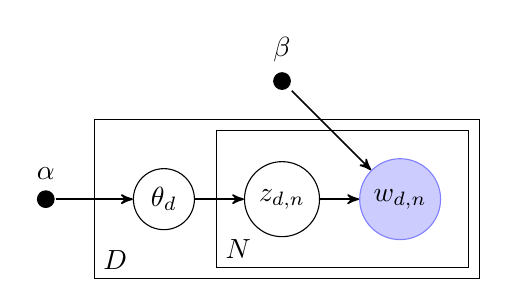
\begin{tikzpicture}
    [
      observed/.style={minimum size=15pt,circle,draw=blue!50,fill=blue!20},
      unobserved/.style={minimum size=15pt,circle,draw},
      hyper/.style={minimum size=1pt,circle,fill=black},
      post/.style={->,>=stealth',semithick},
    ]

    \node (w-j) [observed] at (0,0) {$w_{d,n}$};
    \node (z-j) [unobserved] at (-1.5,0) {$z_{d,n}$};
    \node (z-prior) [unobserved] at (-3,0) {$\theta_d$};
    \node (z-hyper) [label=above:$\alpha$] at (-4.5,0) {};
    \filldraw [black] (-4.5,0) circle (3pt);
    \node (w-hyper) [label=above:$\beta$] at (-1.5,1.5) {};
    \filldraw [black] (-1.5,1.5) circle (3pt);
    
    \path
    (z-j) edge [post] (w-j)
    
    (z-hyper) edge [post] (z-prior)
    (z-prior) edge [post] (z-j)

    (w-hyper) edge [post] (w-j)
    ;

    \node [draw,fit=(w-j) (z-prior), inner sep=14pt] (plate-context) {};
    \node [above right] at (plate-context.south west) {$D$};
    \node [draw,fit=(w-j) (z-j), inner sep=10pt] (plate-token) {};
    \node [above right] at (plate-token.south west) {$N$};

  \end{tikzpicture}
  \caption{Plate Diagram of LDA. For more information, see \citet{Blei:2003:LDA:944919.944937} }
  \label{fig:lda-graphical-model}
\end{figure}

where
\\{$\theta_d$} represents the topic proportions for the \textit{d}th document
\\{$z_{d,n}$} represents the topic assignments for the \textit{n}th word in the \textit{d}th document
\\{$w_{d,n}$} represents the observed word for the \textit{n}th word in the \textit{d}th document
\\{$\beta$} represents a distribution over the words in the known vocabulary

I have considered the LDA topics to be equivalent to the aspects extracted from the reviews. Under this perspective, I have tried to test the hypothesis that reviews created by the same persons using multiple accounts would have similar topic distributions. 

\subsection{Data preprocessing}

For these experiments, I have used the Trustpilot labeled dataset containing 8990 reviews split almost equally between known truthful and deceptive reviews. Similar to the initial experiments, first, I eliminated all the stopwords that appear in the list created by  \citet{SaltonandBuckleyStopWordsAggresive}, then I have used the Stanford Log-linear Part-Of-Speech Tagger \citet{StanfordNLPTagger} to tokenize the reviews and extract only the nouns, verbs and adjectives. After these steps, I computed the frequency of the words in the new corpus and plotted the frequency histogram to check the distribution of the remaining words. The goal was to remove more uninformative, highly seller-specific words, i.e. words with very low frequency, as well as highly frequent words, such as for example \textit{buy}, \text{price} and \textit{service} which occurred more than 2000 times in the 9000 reviews. These words are inducing noise into the topic distribution and could be added to the stopwords list from the initial preprocessing step. Figure \ref{fig:lda-words-hist} in the \nameref{chapter:Results} chapter shows the words distribution before and after the removal of the extra frequent words. 

Furthermore, reviews which did not have at least 10 words after the previous words filtering step were also removed from the corpus, since the quality of the LDA topics is known to be low for short and sparse texts. There were many reviews which after the initial word-frequency filtering ended up having a single word. Each word comes from exactly one topic in LDA, so for one-word documents, it means that one topic would have a very high weight and the other topics would have very low weights. Thus when paired with other reviews, the similarity score would be very low. 

\subsection{Similarity measures}

Each review is a distribution over topics, so computing the similarity between two reviews translates to computing the similarity between their underlying topic distributions. The Kullback-Leibner (KL) \citet{Kullback1951} measures the difference between two probability distributions \textit{P} and \textit{Q} as shown in equation \ref{eq:KL}. So it can be used to compute a value for the distance between the underlying topics distributions of two reviews. This measure has two drawbacks though. If \textit{Q(i)} is zero, then the measure is undefined. It is also not symmetric, meaning the divergence from \textit{P} to \textit{Q} is not the same as that from \textit{Q} to \textit{P}. Translating this to the reviews context, it is not a suitable metric to use, because if a review \textit{$R_1$} is similar to \textit{$R_2$} then it would be expected that \textit{$R_2$} is similar with the same amount to \textit{$R_1$}.

\begin{equation}\label{eq:KL}
KL(P\|Q) = \sum_i \ln\left(\frac{P(i)}{Q(i)}\right) P(i).\!
\end{equation}

The Jensen-Shannon (JS) measure is based on the KL divergence and it addresses these drawbacks: it is symmetric and always provides a finite value. It is also bounded by 1, which is more useful when comparing a similarity value for a review pair with a fixed threshold in order to classify the reviews as fake. Equation \ref{eq:JS} formulates the JS measure.

\begin{equation}\label{eq:JS}
JS(P \parallel Q)= \frac{1}{2}KL(P \parallel M)+\frac{1}{2}KL(Q \parallel M), \hspace{0.2cm} where \hspace{0.2cm} M=\frac{1}{2}(P+Q)
\end{equation}

The JS measure can be rewritten in the form of equation \ref{eq:IR}, in order to decrease computational time for large vocabularies, as mentioned by \citet{dagan1999similarity}. IR is short for information radius, while {$\beta$} is 
a statistical control parameter.

\begin{equation}\label{eq:IR}
IR(P,Q) = 10^{-\beta{JS(P \parallel Q)}}
\end{equation}

The IR measure was applied to all review pairs forming the new corpus, after the data preprocessing step. Similar to the model presented in section \ref{section:singleton-detection}, similarity thresholds were used to validate the output from the review classifier. The validation procedure was the individual review pair strategy presented earlier in section \ref{subsection:validating_classifier_output}, with the small change that instead of applying it to clusters, it was applied to all the reviews from a seller. The computed similarity was then compared to a fixed spam threshold in order to predict whether the reviews were truthful or deceptive. 

The pseudocode above summarizes the method's steps.
\begin{algorithm}
\caption*{Pseudocode for the aspect-based mining for opinion spam detection method}
\label{alg:aspect-mining}
\begin{algorithmic}[1]
	\For{each review $R$ in dataset}
		\State Remove stopwords
	  	\State Extract nouns, verbs and adjectives
  	\EndFor
  	\State Run LDA for \#topics {$\in$} \{10, 30, 50, 70, 100\}
	\For{each \#topics}
	  	\For{each reviews pair ($R_i$, $R_j$)}
		\State $sim(R_i, R_j)$ = $\underset{R_i{\sim}T_i, R_j{\sim}T_j}{similarity\_measure}(T_i, T_j)$
		\EndFor
		\For{$spam\ threshold\ T = 0.5$, $T <= 1$, $T{+=}{0.05}$}
			\If{${sim(R_i, R_j)}$ > ${T}$}
				\State Mark $R_i$ and $R_j$ as deceptive
			\Else 
				\State Mark $R_i$ and $R_j$ as truthful
			\EndIf
		\EndFor
	\EndFor
\end{algorithmic}
\end{algorithm}

I have used the Semilar toolkit to extract the topic distributions for all the reviews and made no changes to the default LDA parameter values set in the toolkit. The number of topics was in the set \{10, 30, 50, 70, 100\}.
The results have been plotted and discussed in the \nameref{chapter:Results} chapter.                                 %Chapter 4
\chapter{Results}
\label{chapter:Results}
\section{Singleton opinion spam detection}

\setkeys{Gin}{width=0.8\textwidth} 


As mentioned in the \nameref{chapter:Method} chapter, I have used two clustering algorithms DBSCAN and OPTICS to create review groups based on the behavioral features. The purpose was to see which algorithm performs best on my dataset and better adapts to the user behavior. 
I have experimented with \textit{epsilon} in \{0.02, 0.05, 0.08, 0.1, 0.4\}. The two marginal values 0.02 and 0.4 produced very high clustering noise, meaning a lot of reviews were not clustered. They also recorded a very low precision and F1 score, so I will not mention them in this section.

Moreover, I have experimented with the cosine similarity including all words (excluding stopwords) and used nouns, verbs and adjectives parts-of-speech for the rest of the measures. The best results were obtained in the following scenarios:
\begin{itemize}
\item cosine similarity with all parts-of-speech tags, excluding stopwords
\item cosine similarity with non-lemmatized POSs - nouns, verbs and adjectives, excluding stopwords
\item cosine similarity with lemmatized POSs - nouns, verbs and adjectives, excluding stopwords
\item mihalcea semantic similarity - nouns, verbs and adjectives, excluding stopwords
\item maxsim - maximum value among of all the previous measures
\end{itemize}
Each candidate review pair compared was labeled as deceptive if it exceeded a certain similarity threshold. The minimum threshold value was set to 0.5 and the maximum value was 1, where 1 would indicate an identical pair of reviews.

The clustering phase managed to produce relevant clusters, although it was based on very simple behavioral features. It also produced a significant amount of noise. For DBSCAN with \textit{epsilon} = 0.1, the classifier performed very well, reaching even precision of over 90\% for higher thresholds. But a very large number of reviews was actually discarded from the similarity model because they were not clustered.

A conclusion would be that very dense review clusters are likely to be the result of a bursty behavior of a user which posts reviews for the same seller in a very short amount of time. This is a very obvious type of opinion spam, when the user usually also copy-pastes a large portion of the text between reviews. Upon manual inspection of the reviews in the clusters leading to such high precision, I could verify the reviews were indeed close to identical.

The DBSCAN approach offered good results using the cluster validation strategy. For \textit{epsilon} = 0.1 and minPts = 2, it achieved a precision of  90\% at thresholds larger than 0.85 for all the similarity measures, as Figure \ref{fig:dbscan-minpts-2-eps-0-1-precision-cluster} shows. The results were even better when the individual validation strategy was applied and the precision reached 90\% even with a threshold of 0.75 as Figure \ref{fig:dbscan-minpts-2-eps-0-1-precision-individual} shows. It can be observed that the precision of the semantic measure is generally very close or higher than that of the vectorial measures above a threshold of 0.7. The intuition that the scores should become more precise as the threshold is raised is proven by the results. Also in a production system, the threshold value can easily be tuned to achieve a desired precision.

The noise produced by DBSCAN was around 30\% for \textit{epsilon} = 0.1, meaning if a seller had 99 reviews, 33 of them were discarded because they did not end up in any cluster. The noise increased as \textit{epsilon} was lowered to 0.08 and 0.05. The semantic method outperformed all the others in terms of recall and scored at least double the value of the vectorial measures in the case of the cluster validation strategy for lower thresholds. It scored three times higher than the other measures for the individual review pair validation as shown in Table \ref{tab:dbscan-minpts-2-eps-0-1-cluster} and Table \ref{tab:dbscan-minpts-2-eps-0-1-individual}. 

The OPTICS algorithm produced significantly less noise than DBSCAN because of its ability to adjust to density variations much better. It managed to cluster a very large portion of the dataset and thus more review pairs could be measured for similarity. Figure \ref{optics-minpts-2} shows the precision reached 80\%, above a similarity threshold of 0.75, which is 10\% lower than for DBSCAN. The recall and F1 scores achieved are also lower. For the semantic measure, it provided a F1 score of only 24\% for a precision of 68\% at a threshold of 0.7, compared to DBSCAN which got an almost double F1 score of 47\% and a precision of 70\% for the same threshold.

The semantic measure achieved a better F1 score than the vectorial measures and this proves that semantic similarity outperforms cosine similarity in the detection of deceptive singleton reviews. 
Generally, the F1 score obtained through the cluster validation strategy is higher than with the individual review pair validation because of the strategy's granularity. All the reviews of the cluster are considered deceptive if at least one review pair goes over the similarity threshold. So, although naturally the first strategy is less precise, it proves that more deceptive reviews surface when a grouping is applied even on straightforward features such as rating and date. 

As noted earlier in the \nameref{chapter:Method} chapter, the purpose of the \textit{maxsim} similarity measure is to try and make the best of both worlds - vectorial and semantic. Although intuitively, the semantic similarity should always outperform the vectorial counterpart since every word should be semantically identical first of all to itself, results have shown that there are times when the cosine similarity gives better precision in relation to the classifier validation techniques used than the semantic approach. 

\textit{Maxsim} scored almost identically to the semantic similarity measure, in terms of precision and recall, with recall being constantly 1\% better for all \textit{epsilon} values. It also achieved the best F1 score, thus outperforming the cosine vectorial method and very slightly the semantic similarity. In order to avoid cluttering the figures, \textit{maxsim} has not been plotted, but its results are shown in Tables \ref{tab:dbscan-minpts-2-eps-0-1-cluster} - \ref{tab:optics-minpts-2-individual}.

Figures \ref{dbscan-minpts-2-eps-0-1} - \ref{optics-minpts-2} show the classifier precision and F1 score obtained for all the similarity measures, with DBSCAN's input parameters (\textit{epsilon} in \{0.05, 0.08, 0.1\}, \textit{minPts} = 2) and OPTICS with \textit{minPts} = 2.

This chapter includes the results tables for DBSCAN with \textit{epsilon} = 0.1 and OPTICS, while the rest of the results tables for other \textit{epsilon} values can be seen in the \nameref{chapter:Appendix}.

\begin{figure}[ht]
\begin{center}
\subfloat[Subfigure 1 list of figures text][Precision - cluster validation strategy]{
\includegraphics[width=0.5\textwidth]{sweave/sweave-dbscan-minpts-2-eps-0-1-cluster-precision}
\label{fig:dbscan-minpts-2-eps-0-1-precision-cluster}}
\subfloat[Subfigure 2 list of figures text][F1 score - cluster validation strategy]{
\includegraphics[width=0.5\textwidth]{sweave/sweave-dbscan-minpts-2-eps-0-1-cluster-f1score}
\label{fig:dbscan-minpts-2-eps-0-1-f1score-cluster}}
\qquad
\subfloat[Subfigure 3 list of figures text][Precision - individual validation strategy]{
\includegraphics[width=0.5\textwidth]{sweave/sweave-dbscan-minpts-2-eps-0-1-individual-precision}
\label{fig:dbscan-minpts-2-eps-0-1-precision-individual}}
\subfloat[Subfigure 4 list of figures text][F1 score - individual validation strategy]{
\includegraphics[width=0.5\textwidth]{sweave/sweave-dbscan-minpts-2-eps-0-1-individual-f1score}
\label{fig:dbscan-minpts-2-eps-0-1-f1score-individual}}
\caption{Classifier precision and F1 score for DBSCAN with minPts=2 and epsilon=0.1 using both the cluster and the individual review pair validation strategies}    
\label{dbscan-minpts-2-eps-0-1}
\end{center}
\end{figure}

\begin{figure}[ht]
\begin{center}
\subfloat[Subfigure 1 list of figures text][Precision - cluster validation strategy]{
\includegraphics[width=0.5\textwidth]{sweave/sweave-dbscan-minpts-2-eps-0-08-cluster-precision}
\label{fig:subfig1}}
\subfloat[Subfigure 2 list of figures text][F1 score - cluster validation strategy]{
\includegraphics[width=0.5\textwidth]{sweave/sweave-dbscan-minpts-2-eps-0-08-cluster-f1score}
\label{fig:subfig2}}
\qquad
\subfloat[Subfigure 3 list of figures text][Precision - individual validation strategy]{
\includegraphics[width=0.5\textwidth]{sweave/sweave-dbscan-minpts-2-eps-0-08-individual-precision}
\label{fig:subfig3}}
\subfloat[Subfigure 4 list of figures text][F1 score - individual validation strategy]{
\includegraphics[width=0.5\textwidth]{sweave/sweave-dbscan-minpts-2-eps-0-08-individual-f1score}
\label{fig:subfig4}}
\caption{Classifier precision and F1 score for DBSCAN with minPts=2 and epsilon=0.08 using both the cluster and the individual review pair validation strategies}    
\label{dbscan-minpts-2-eps-0-08}
\end{center}
\end{figure}

\begin{figure}[ht]
\begin{center}
\subfloat[Subfigure 1 list of figures text][Precision - cluster validation strategy]{
\includegraphics[width=0.5\textwidth]{sweave/sweave-dbscan-minpts-2-eps-0-05-cluster-precision}
\label{fig:subfig1}}
\subfloat[Subfigure 2 list of figures text][F1 score - cluster validation strategy]{
\includegraphics[width=0.5\textwidth]{sweave/sweave-dbscan-minpts-2-eps-0-05-cluster-f1score}
\label{fig:subfig2}}
\qquad
\subfloat[Subfigure 3 list of figures text][Precision - individual validation strategy]{
\includegraphics[width=0.5\textwidth]{sweave/sweave-dbscan-minpts-2-eps-0-05-individual-precision}
\label{fig:subfig3}}
\subfloat[Subfigure 4 list of figures text][F1 score - individual validation strategy]{
\includegraphics[width=0.5\textwidth]{sweave/sweave-dbscan-minpts-2-eps-0-05-individual-f1score}
\label{fig:subfig4}}
\caption{Classifier precision and F1 score for DBSCAN with minPts=2 and epsilon=0.05 using both the cluster and the individual review pair validation strategies}    
\label{dbscan-minpts-2-eps-0-05}
\end{center}
\end{figure}

\begin{figure}[ht]
\begin{center}
\subfloat[Subfigure 1 list of figures text][Precision - cluster validation strategy]{
\includegraphics[width=0.5\textwidth]{sweave/sweave-optics-minpts-2-cluster-precision}
\label{fig:subfig1}}
\subfloat[Subfigure 2 list of figures text][F1 score - cluster validation strategy]{
\includegraphics[width=0.5\textwidth]{sweave/sweave-optics-minpts-2-cluster-f1score}
\label{fig:subfig2}}
\qquad
\subfloat[Subfigure 3 list of figures text][Precision - individual validation strategy]{
\includegraphics[width=0.5\textwidth]{sweave/sweave-optics-minpts-2-individual-precision}
\label{fig:subfig3}}
\subfloat[Subfigure 4 list of figures text][F1 score - individual validation strategy]{
\includegraphics[width=0.5\textwidth]{sweave/sweave-optics-minpts-2-individual-f1score}
\label{fig:subfig4}}
\caption{Classifier precision and F1 score for OPTICS with minPts=2 using both the cluster and the individual review pair validation strategies}    
\label{optics-minpts-2}
\end{center}
\end{figure}

\clearpage
The exact numbers behind the previous plots for both DBSCAN and OPTICS clustering algorithms are shown in Tables \ref{tab:dbscan-minpts-2-eps-0-1-cluster} - \ref{tab:optics-minpts-2-individual}. 

Table \ref{tab:legend} describes the short names used for the columns in each of the results tables. 

\begin{table}[h]
\begin{center}
    \begin{tabular}{ | p{0.2\textwidth} | p{0.7\textwidth} |}
    \hline
    \textbf{Column} & \textbf{Description} \\ \hline
    T & threshold  \\ \hline
    cos & cosine similarity with all parts-of-speech tags, excluding stopwords \\ \hline
    cpnl & cosine similarity with only non-lemmatized POS - nouns, verbs and adjectives, excluding stopwords \\ \hline
    cpl & cosine similarity with only lemmatized POS - combinations between nouns, verbs and adjectives, excluding stopwords \\ \hline
    mih & mihalcea semantic similarity - combinations between nouns, verbs and adjectives, excluding stopwords\\ \hline
    max & \textit{maxsim} - maximum value among of all the previous measures \\ \hline
    P/R/A/F & precision/recall/accuracy/F1-score \\ \hline
    \end{tabular}
\caption{Description of the column names used in the results tables}
\label{tab:legend}
\end{center}
\end{table}
\begin{center}
% latex table generated in R 3.0.2 by xtable 1.7-3 package
% Sat May 17 18:59:54 2014
\begin{table}[!h]
\centering
\begin{tabular}{|l|l|l|l|l|l|l|l|l|l|l|}
  \hline
T & cos & cos & cos & cos & cpnl & cpnl & cpnl & cpnl & cpl & cpl \\ 
  \hline
T & P & R & A & F & P & R & A & F & P & R \\ 
   \hline
0.5 & 0.70 & 0.50 & 0.53 & 0.58 & 0.68 & 0.41 & 0.49 & 0.51 & 0.71 & 0.48 \\ 
  0.6 & 0.72 & 0.34 & 0.48 & 0.46 & 0.79 & 0.24 & 0.46 & 0.37 & 0.70 & 0.36 \\ 
  0.7 & 0.75 & 0.18 & 0.42 & 0.29 & 0.74 & 0.14 & 0.40 & 0.24 & 0.76 & 0.19 \\ 
  0.8 & 0.86 & 0.12 & 0.41 & 0.22 & 0.81 & 0.11 & 0.40 & 0.20 & 0.69 & 0.12 \\ 
  0.9 & 0.90 & 0.10 & 0.40 & 0.18 & 0.90 & 0.10 & 0.40 & 0.18 & 0.90 & 0.10 \\ 
   \hline
\end{tabular}
\end{table}
% latex table generated in R 3.0.2 by xtable 1.7-3 package
% Sat May 17 18:59:54 2014
\begin{table}[!h]
\centering
\begin{tabular}{|l|l|l|l|l|l|l|l|l|l|l|}
  \hline
T & cpl & cpl & mih & mih & mih & mih & max & max & max & max \\ 
  \hline
T & A & F & P & R & A & F & P & R & A & F \\ 
   \hline
0.5 & 0.53 & 0.57 & 0.69 & 0.80 & 0.63 & 0.74 & 0.69 & 0.81 & 0.63 & 0.74 \\ 
  0.6 & 0.48 & 0.48 & 0.70 & 0.60 & 0.57 & 0.65 & 0.70 & 0.61 & 0.57 & 0.65 \\ 
  0.7 & 0.43 & 0.30 & 0.70 & 0.36 & 0.47 & 0.47 & 0.70 & 0.36 & 0.48 & 0.47 \\ 
  0.8 & 0.39 & 0.21 & 0.80 & 0.12 & 0.40 & 0.21 & 0.71 & 0.15 & 0.40 & 0.24 \\ 
  0.9 & 0.40 & 0.18 & 0.91 & 0.10 & 0.40 & 0.19 & 0.91 & 0.10 & 0.40 & 0.19 \\ 
   \hline
\end{tabular}
\caption{Classifier results for DBSCAN with minPts=2, epsilon=0.1 using the cluster validation strategy} 
\label{tab:dbscan-minpts-2-eps-0-1-cluster}
\end{table}\end{center}

\begin{center}
% latex table generated in R 3.0.2 by xtable 1.7-3 package
% Sat May 17 18:59:54 2014
\begin{table}[!h]
\centering
\begin{tabular}{|l|l|l|l|l|l|l|l|l|l|l|}
  \hline
T & cos & cos & cos & cos & cpnl & cpnl & cpnl & cpnl & cpl & cpl \\ 
  \hline
T & P & R & A & F & P & R & A & F & P & R \\ 
   \hline
0.5 & 0.75 & 0.16 & 0.40 & 0.27 & 0.72 & 0.09 & 0.38 & 0.16 & 0.75 & 0.15 \\ 
  0.6 & 0.78 & 0.07 & 0.37 & 0.13 & 0.79 & 0.04 & 0.36 & 0.07 & 0.75 & 0.07 \\ 
  0.7 & 0.83 & 0.03 & 0.36 & 0.06 & 0.84 & 0.03 & 0.35 & 0.05 & 0.84 & 0.03 \\ 
  0.8 & 0.87 & 0.02 & 0.35 & 0.05 & 0.88 & 0.02 & 0.35 & 0.04 & 0.84 & 0.02 \\ 
  0.9 & 0.89 & 0.02 & 0.35 & 0.04 & 0.89 & 0.02 & 0.35 & 0.04 & 0.89 & 0.02 \\ 
   \hline
\end{tabular}
\end{table}
% latex table generated in R 3.0.2 by xtable 1.7-3 package
% Sat May 17 18:59:54 2014
\begin{table}[!h]
\centering
\begin{tabular}{|l|l|l|l|l|l|l|l|l|l|l|}
  \hline
T & cpl & cpl & mih & mih & mih & mih & max & max & max & max \\ 
  \hline
T & A & F & P & R & A & F & P & R & A & F \\ 
   \hline
0.5 & 0.40 & 0.25 & 0.70 & 0.41 & 0.48 & 0.52 & 0.70 & 0.42 & 0.48 & 0.52 \\ 
  0.6 & 0.37 & 0.13 & 0.73 & 0.23 & 0.43 & 0.35 & 0.72 & 0.24 & 0.43 & 0.36 \\ 
  0.7 & 0.36 & 0.06 & 0.79 & 0.07 & 0.37 & 0.12 & 0.79 & 0.07 & 0.37 & 0.13 \\ 
  0.8 & 0.35 & 0.05 & 0.85 & 0.02 & 0.35 & 0.05 & 0.84 & 0.03 & 0.35 & 0.05 \\ 
  0.9 & 0.35 & 0.04 & 0.90 & 0.02 & 0.35 & 0.04 & 0.90 & 0.02 & 0.35 & 0.04 \\ 
   \hline
\end{tabular}
\caption{Classifier results for DBSCAN with minPts=2, epsilon=0.1 using the individual review pair validation strategy} 
\label{tab:dbscan-minpts-2-eps-0-1-individual}
\end{table}\end{center}
\begin{center}
% latex table generated in R 3.0.2 by xtable 1.7-3 package
% Sat May 17 18:59:54 2014
\begin{table}[!h]
\centering
\begin{tabular}{|l|l|l|l|l|l|l|l|l|l|l|}
  \hline
T & cos & cos & cos & cos & cpnl & cpnl & cpnl & cpnl & cpl & cpl \\ 
  \hline
T & P & R & A & F & P & R & A & F & P & R \\ 
   \hline
0.5 & 0.62 & 0.30 & 0.48 & 0.41 & 0.63 & 0.18 & 0.46 & 0.28 & 0.64 & 0.29 \\ 
  0.6 & 0.69 & 0.16 & 0.46 & 0.26 & 0.57 & 0.08 & 0.42 & 0.14 & 0.66 & 0.15 \\ 
  0.7 & 0.77 & 0.06 & 0.44 & 0.11 & 0.63 & 0.05 & 0.42 & 0.09 & 0.76 & 0.06 \\ 
  0.8 & 0.75 & 0.05 & 0.43 & 0.09 & 0.76 & 0.05 & 0.43 & 0.09 & 0.73 & 0.05 \\ 
  0.9 & 0.74 & 0.04 & 0.43 & 0.08 & 0.74 & 0.04 & 0.43 & 0.08 & 0.74 & 0.04 \\ 
   \hline
\end{tabular}
\end{table}
% latex table generated in R 3.0.2 by xtable 1.7-3 package
% Sat May 17 18:59:54 2014
\begin{table}[!h]
\centering
\begin{tabular}{|l|l|l|l|l|l|l|l|l|l|l|}
  \hline
T & cpl & cpl & mih & mih & mih & mih & max & max & max & max \\ 
  \hline
T & A & F & P & R & A & F & P & R & A & F \\ 
   \hline
0.5 & 0.49 & 0.40 & 0.59 & 0.75 & 0.55 & 0.66 & 0.59 & 0.76 & 0.55 & 0.67 \\ 
  0.6 & 0.45 & 0.25 & 0.59 & 0.41 & 0.49 & 0.49 & 0.59 & 0.43 & 0.49 & 0.50 \\ 
  0.7 & 0.43 & 0.11 & 0.68 & 0.15 & 0.46 & 0.24 & 0.69 & 0.15 & 0.46 & 0.25 \\ 
  0.8 & 0.43 & 0.09 & 0.75 & 0.05 & 0.43 & 0.10 & 0.74 & 0.05 & 0.43 & 0.10 \\ 
  0.9 & 0.43 & 0.08 & 0.76 & 0.05 & 0.43 & 0.09 & 0.76 & 0.05 & 0.43 & 0.09 \\ 
   \hline
\end{tabular}
\caption{Classifier results for OPTICS with minPts=2 using the cluster validation strategy} 
\label{tab:optics-minpts-2-cluster}
\end{table}\end{center}
\begin{center}
% latex table generated in R 3.0.2 by xtable 1.7-3 package
% Sat May 17 18:59:54 2014
\begin{table}[!h]
\centering
\begin{tabular}{|l|l|l|l|l|l|l|l|l|l|l|}
  \hline
T & cos & cos & cos & cos & cpnl & cpnl & cpnl & cpnl & cpl & cpl \\ 
  \hline
T & P & R & A & F & P & R & A & F & P & R \\ 
   \hline
0.5 & 0.71 & 0.11 & 0.44 & 0.19 & 0.73 & 0.06 & 0.43 & 0.11 & 0.72 & 0.11 \\ 
  0.6 & 0.74 & 0.04 & 0.42 & 0.08 & 0.71 & 0.02 & 0.42 & 0.05 & 0.72 & 0.04 \\ 
  0.7 & 0.81 & 0.02 & 0.42 & 0.04 & 0.75 & 0.02 & 0.42 & 0.03 & 0.77 & 0.02 \\ 
  0.8 & 0.76 & 0.02 & 0.41 & 0.03 & 0.80 & 0.01 & 0.42 & 0.03 & 0.76 & 0.02 \\ 
  0.9 & 0.78 & 0.01 & 0.41 & 0.03 & 0.78 & 0.01 & 0.41 & 0.03 & 0.78 & 0.01 \\ 
   \hline
\end{tabular}
\end{table}
% latex table generated in R 3.0.2 by xtable 1.7-3 package
% Sat May 17 18:59:54 2014
\begin{table}[!h]
\centering
\begin{tabular}{|l|l|l|l|l|l|l|l|l|l|l|}
  \hline
T & cpl & cpl & mih & mih & mih & mih & max & max & max & max \\ 
  \hline
T & A & F & P & R & A & F & P & R & A & F \\ 
   \hline
0.5 & 0.44 & 0.19 & 0.60 & 0.38 & 0.49 & 0.46 & 0.60 & 0.38 & 0.49 & 0.47 \\ 
  0.6 & 0.42 & 0.08 & 0.66 & 0.18 & 0.45 & 0.28 & 0.65 & 0.19 & 0.45 & 0.29 \\ 
  0.7 & 0.42 & 0.04 & 0.71 & 0.03 & 0.42 & 0.07 & 0.72 & 0.04 & 0.42 & 0.07 \\ 
  0.8 & 0.42 & 0.03 & 0.76 & 0.02 & 0.41 & 0.03 & 0.76 & 0.02 & 0.42 & 0.03 \\ 
  0.9 & 0.41 & 0.03 & 0.78 & 0.01 & 0.41 & 0.03 & 0.78 & 0.01 & 0.41 & 0.03 \\ 
   \hline
\end{tabular}
\caption{Classifier results for OPTICS with minPts=2 using the individual review pair validation strategy} 
\label{tab:optics-minpts-2-individual}
\end{table}\end{center}

\clearpage 

\section{Distribution of truthful and deceptive reviews}

The CDF curves plotted in Figures \ref{fig:cdf_trustpilot} - \ref{fig:cdf_ott} reveal several interesting aspects. They show the amount of content similarity for the truthful/fake reviews taken separately as well as the position and bounds for each type and the gaps between the two curves. Regardless of the type of similarity measure used, i.e. vectorial or semantic, the two distributional curves of truthful and fake reviews are clearly separated. For the truthful reviews (blue color), the curve appears towards the left of the plot, while for the fake reviews (red color) it is more towards the right. This means that for any similarity measure applied, for a fixed cumulative percentage value, its corresponding value \textit{$x_t$} for truthful reviews will be lower than the value for deceptive reviews \textit{$x_d$}. 

Figure \ref{fig:cdf_trustpilot_mihalcea} shows the largest discriminative margin between the two curves recorded for the Trustpilot dataset. For example, for a fixed cumulative percentage value of 0.4, 40\% of truthful reviews are bounded by a semantic similarity of only 0.28, compared to the same percentage of fake reviews which are bounded by a similarity value of 0.4. For a cumulative percentage of 0.8, 80\% of truthful reviews are bounded by a semantic similarity value of 0.43, while the fake reviews by 0.52. 

In the case of the Ott dataset, Figure \ref{fig:cdf_ott_mihalcea} shows that for a fixed cumulative percentage value of 0.4, 40\% of truthful reviews are bounded by a semantic similarity of only 0.22, compared to the same percentage of fake reviews which are bounded by a similarity value of 0.32. For a cumulative percentage of 0.8, 80\% of truthful reviews are bounded by a semantic similarity value of 0.38, while the fake reviews by 0.44. 

This shows that people writing deceptive reviews tend to have a higher semantic similarity between their reviews than the users writing honest reviews, probably because they are the same person under multiple accounts or know each other and work together. The honest users do not influence each other's writing style so much. The spammers are more likely to do that.

It appears that in both datasets, this gap is not so prominent for the cosine-based measures and this shows that by using the vectorial measures, it becomes harder to differentiate between the truthful and the deceptive reviews. For the Trustpilot dataset, Figure \ref{fig:cdf_trustpilot_cosine} shows that 40\% of truthful reviews are bounded by a cosine similarity value of 0.08, compared to only 0.1 for fake reviews. The difference of 0.02 is significantly lower then the semantic measure which showed a larger gap of 0.12. 

\begin{figure}[ht]
\begin{center}
\subfloat[Subfigure 1 list of figures text][Mihalcea]{
\includegraphics[width=0.5\textwidth]{sweave/sweave-trustpilotmihalceacdf}
\label{fig:cdf_trustpilot_mihalcea}}
\subfloat[Subfigure 2 list of figures text][Cosine]{
\includegraphics[width=0.5\textwidth]{sweave/sweave-trustpilotcosinecdf}
\label{fig:cdf_trustpilot_cosine}}
\qquad
\subfloat[Subfigure 3 list of figures text][Cosine without lemmatization]{
\includegraphics[width=0.5\textwidth]{sweave/sweave-trustpilotcosineposnonlemmatizedcdf}
\label{fig:cdf_trustpilot_cosineposnonlemmatized}}
\subfloat[Subfigure 4 list of figures text][Cosine with lemmatization]{
\includegraphics[width=0.5\textwidth]{sweave/sweave-trustpilotcosineposlemmatizedcdf}
\label{fig:cdf_trustpilot_cosineposlemmatized}}
\caption{Trustpilot dataset - cumulative percentage of fake reviews (red color) and truthful reviews (blue color) vs. similarity measures values}    
\label{fig:cdf_trustpilot}
\end{center}
\end{figure}

\begin{figure}[ht]
\begin{center}
\subfloat[Subfigure 1 list of figures text][Mihalcea]{
\includegraphics[width=0.5\textwidth]{sweave/sweave-ottmihalcea}
\label{fig:cdf_ott_mihalcea}}
\subfloat[Subfigure 2 list of figures text][Cosine]{
\includegraphics[width=0.5\textwidth]{sweave/sweave-ottcosine}
\label{fig:cdf_ott_cosine}}
\qquad
\subfloat[Subfigure 3 list of figures text][Cosine without lemmatization]{
\includegraphics[width=0.5\textwidth]{sweave/sweave-ottcosineposnonlemmatized}
\label{fig:cdf_ott_cosine_without_lemmatization}}
\subfloat[Subfigure 4 list of figures text][Cosine with lemmatization]{
\includegraphics[width=0.5\textwidth]{sweave/sweave-ottcosineposlemmatized}
\label{fig:cdf_ott_cosine_with_lemmatization}}
\caption{Ott dataset - cumulative percentage of fake reviews (red color) and truthful reviews (blue color) vs. similarity measures values}    
\label{fig:cdf_ott}
\end{center}
\end{figure}

\clearpage 

For the Ott dataset, Figure \ref{fig:cdf_ott_cosine} shows that 80\% of truthful reviews are bounded by a cosine similarity value of 0.32, compared to the 0.34 for fake reviews. The difference is only of 0.2 compared to the semantic similarity measure which showed a gap of 0.6. An even smaller difference can be seen for the cosine with and without lemmatization measures. 

Another interesting aspect observed in the Trustpilot dataset is the steep initial jump of the vectorial measures. The cosine without lemmatization measure in Figure \ref{fig:cdf_trustpilot_cosineposnonlemmatized} shows that almost 25\% of the fake reviews exhibit zero similarity between each other. For the same cumulative percentage, the semantic measure shows a similarity bound of up to 0.32. The cosine and cosine with lemmatization measures in Figures \ref{fig:cdf_trustpilot_cosine} - \ref{fig:cdf_trustpilot_cosineposlemmatized} have a similar distribution with a clear but small gap between the curves with about 50\% of known deceptive reviews having a similarity bound of 0.2. Compared to the semantic measure, only 10\% of the fake reviews have a similarity below this value.

One obvious question is why isn't this gap larger, especially for the semantic similarity measure, regardless of the dataset? 

One possible explanation might be that reviews from the same seller generally talk pretty much about aspects within a very specific context, which is related to the shop's business area of activity. For example, if the shop is an electronics reseller that offers online ordering, home delivery and customer support for sold items, then the review will probably contain aspects related to website, the delivery speed, customer support, service level, screen, battery, price and so on. It is pretty easy for the spammers to mimic the honest reviews in the sense of mentioning the same key aspects in their reviews.

The dataset of \citet{Ott2011} has been created using Amazon Mechanical Turk (AMT), so it is likely the turkers was separate persons and did not know each other. It is a different setup than for the real-life Trustpilot dataset, where the fake reviews are more likely to be written by the same people using multiple accounts on the review platform. \citet{Mukherjee2013a} questioned the validity of using fake reviews obtained through a crowdsourcing service such as AMT to detect real-life deceptive reviews in a commercial website and their results showed a much lower accuracy when testing on real-life Yelp reviews than what \citet{Ott2011} reported in their study. 

To conclude, two other possible explanations for why the gap is not larger might be that first of all, the AMT users were separate persons and second, the crowdsourced data may not be representative of real-life scenarios. 

\clearpage

\section{Aspect-based mining for opinion spam detection}

Figure \ref{fig:lda-words-all-hist} shows the long tail distribution of all the words frequencies.  Figure \ref{fig:lda-words-3-100-hist} shows the log-histogram resulted after filtering out words that appeared either at most twice or more than 100 times in the review corpus. Although the distribution still has a positive skew, the filtering step has managed to improve the similarity results significantly, as it will be shown further on in this section. 

The initial LDA model by \citet{Blei:2003:LDA:944919.944937} was ran on a corpus made up of articles from \textit{Science} magazine. These are relatively long English texts about various scientific themes, carefully edited to avoid misspelled words. It can be argued that the distribution tail of consumer reviews is longer than in the initial LDA model applied to edited articles from \textit{Science} magazine, since user reviews are short unedited texts, which can also contain misspelled words. Reviews are also not about varied themes, as the scientific articles, but tend to contain highly frequent words as Table \ref{tab:wordfreq} in the \nameref{chapter:Appendix} shows.

\begin{figure}[ht]
\begin{center}
\subfloat[Subfigure 1 list of figures text][all words]{
\includegraphics[width=0.5\textwidth]{sweave/sweave-lda-words-all-hist}
\label{fig:lda-words-all-hist}}
\subfloat[Subfigure 2 list of figures text][words with a frequency between 3 and 100]{
\includegraphics[width=0.5\textwidth]{sweave/sweave-lda-words-3-100-hist}
\label{fig:lda-words-3-100-hist}}
\qquad
\caption{Log-histogram for the words frequencies}    
\label{fig:lda-words-hist}
\end{center}
\end{figure}

I have manually checked the topics resulted after running the LDA model on the review corpus and they look logically coherent. The classifier results can be seen in Figure \ref{fig:lda}, where only the results for the IR measure were plotted. IR10 refers to the measure applied for 10 topics, IR30 means 30 topics and so on.

\begin{figure}[ht]
\begin{center}
\subfloat[Subfigure 1 list of figures text][Precision]{
\includegraphics[width=0.5\textwidth]{sweave/sweave-lda-precision}
\label{fig:lda_precision}}
\subfloat[Subfigure 2 list of figures text][Recall]{
\includegraphics[width=0.5\textwidth]{sweave/sweave-lda-recall}
\label{fig:lda_recall}}
\qquad
\begin{center}
\subfloat[Subfigure 3 list of figures text][F1 Score]{
\includegraphics[width=0.5\textwidth]{sweave/sweave-lda-f1score}
\label{fig:lda_f1score}}
\end{center}
\caption{Classifier results for the information radius similarity measure}    
\label{fig:lda}
\end{center}
\end{figure}

\clearpage

Figure \ref{fig:lda_precision} shows the precision according to each value of the spam threshold. IR30 (IR measure for 30 topics) scored best and although the precision is not monotonic, generally it does not register significant drops as the threshold is increased. For thresholds of at least 0.7, it remains above 70\% and it peaks at 98\% for a 0.95 threshold. The model does not do so well for the other number of topics and registers significant drops in precision as the threshold is increased. 

The recall and F1 score values are consistent in relation to the number of topics. As the number of topics is increased, the model's performance decreases. The similarity results for 10 topics show the best F1 score, but the precision is more or less a flat line at 65\%. This could happen because 10 topics are way to little to summarize what people say about a seller. 

Table \ref{tab:lda} shows the precision, recall and F1 score of the classifier and the two gray lines indicate the threshold where both IR30 and IR50 scored best in terms of precision. The precision is lower but actually not far than that obtained using the semantic and vectorial similarity measures in the singleton opinion spam detection method, shown in Table \ref{tab:dbscan-minpts-2-eps-0-1-individual}. 

\begin{center}
% latex table generated in R 3.0.2 by xtable 1.7-3 package
% Sat May 17 18:59:54 2014
\begin{table}[!h]
\centering
\begin{tabular}{|l|l|l|l|l|l|l|l|l|l|}
  \hline
T & IR10 & IR10 & IR10 & IR30 & IR30 & IR30 & IR50 & IR50 & IR50 \\ 
  \hline
T & P & R & F & P & R & F & P & R & F \\ 
   \hline
0.2 & 0.65 & 0.58 & 0.61 & 0.65 & 0.49 & 0.56 & 0.65 & 0.41 & 0.51 \\ 
  0.25 & 0.65 & 0.54 & 0.59 & 0.65 & 0.48 & 0.55 & 0.64 & 0.33 & 0.44 \\ 
  0.30 & 0.65 & 0.52 & 0.58 & 0.65 & 0.47 & 0.54 & 0.64 & 0.25 & 0.36 \\ 
  0.35 & 0.65 & 0.51 & 0.57 & 0.64 & 0.43 & 0.52 & 0.62 & 0.16 & 0.26 \\ 
  0.40 & 0.65 & 0.50 & 0.57 & 0.64 & 0.39 & 0.48 & 0.62 & 0.11 & 0.19 \\ 
  0.45 & 0.65 & 0.50 & 0.56 & 0.62 & 0.31 & 0.42 & 0.63 & 0.09 & 0.15 \\ 
  0.50 & 0.65 & 0.50 & 0.56 & 0.60 & 0.23 & 0.34 & 0.64 & 0.06 & 0.12 \\ 
  0.55 & 0.65 & 0.50 & 0.56 & 0.60 & 0.18 & 0.27 & 0.64 & 0.04 & 0.08 \\ 
  0.60 & 0.65 & 0.49 & 0.56 & 0.61 & 0.12 & 0.20 & 0.70 & 0.03 & 0.06 \\ 
  0.65 & 0.65 & 0.49 & 0.56 & 0.63 & 0.09 & 0.16 & 0.76 & 0.03 & 0.05 \\ 
   \rowcolor[gray]{.7} 0.70 & 0.65 & 0.48 & 0.55 & 0.74 & 0.06 & 0.11 & 0.74 & 0.02 & 0.04 \\ 
  0.75 & 0.65 & 0.46 & 0.54 & 0.69 & 0.03 & 0.06 & 0.77 & 0.01 & 0.03 \\ 
   \rowcolor[gray]{.7} 0.80 & 0.66 & 0.41 & 0.51 & 0.77 & 0.02 & 0.05 & 0.75 & 0.01 & 0.03 \\ 
  0.85 & 0.66 & 0.32 & 0.43 & 0.71 & 0.01 & 0.03 & 0.70 & 0.01 & 0.02 \\ 
  0.90 & 0.63 & 0.19 & 0.29 & 0.73 & 0.01 & 0.02 & 0.57 & 0.01 & 0.01 \\ 
  0.95 & 0.67 & 0.05 & 0.10 & 1.00 & 0.01 & 0.01 & 0.50 & 0.00 & 0.00 \\ 
   \hline
\end{tabular}
\caption{Classifier results for LDA model} 
\label{tab:lda}
\end{table}\end{center}

Figure \ref{fig:lda-appendix-5-100-words} in the \nameref{chapter:Appendix} shows the classifier's performance when using words with a frequency between 5 and 100, having the log-histogram plotted in Figure \ref{fig:lda-words-hist-5-100-appendix}. Only reviews having at least 10 words after the word-frequency filtering step were considered. 
                                 %Chapter 5
\chapter{Discussion}\label{chapter:discussion}

In recent years, online reviews have increasingly become a very important resource for consumers when making purchases. The incentive for companies to try to produce fake reviews to boost sales is also growing. It is becoming more and more difficult for people to make well-informed buying decisions without being deceived by the spammers. 

The opinion spam problem was formulated for the first time only a few years ago, but it has quickly become a captivating research area due to the abundance of user-generated reviews which are increasingly having a bigger impact on online purchases. 

In this thesis, I focused on the problem of detecting opinion spam and proposed two methods which were not previously used in this problem context. In chapters \ref{chapter:introduction}, \ref{chapter:goal} and \ref{chapter:relatedwork}, I defined and motivated the research problem and reviewed the existing approaches in the literature. In section \ref{section:singleton-detection} I proposed a detection method based on semantic similarity, which uses WordNet to compute the relatedness between words. Variants of the cosine similarity were also introduced, as well as a new similarity measure \textit{maxsim}, aimed to give the best results from both vectorial and semantic measures. Experimental results showed that semantic similarity can outperform the vectorial model in detecting deceptive reviews, capturing even more subtle textual clues. The precision score of the review classifier showed high results, enough to make the method viable to be integrated in a production detection system.

In such a system, a critical requirement would be how fast it can analyze all incoming reviews for possible similarity against existing reviews. It is practically unfeasible to compare the text of any two opinions for a seller which has thousands of reviews. As a novel contribution, I have proposed to use density-based clustering to group reviews using simple behavioral features, proven to be linked to suspicious user activity. I have made a comparison between the quality of the clusters obtained using two algorithms - DBSCAN and OPTICS - and measured the impact tuning different input parameters has on the overall classifier results, for this problem. I have argued the noise generated by the clustering is not negligible and should be minimized as much as possible by using more well-crafted behavioral features.

In section \ref{section:distribution-reviews} I compared the distributions of truthful and deceptive reviews in both Trustpilot and Ott datasets. The first contains only real-life reviews while Ott's dataset contains real-life truthful reviews from TripAdvisor and crowdsourced deceptive reviews. It appears that in both datasets, the gap between the distributional curves of the two review types is not so prominent for the cosine-based measures as it is for the semantic one. This supports the hypothesis that it is harder to differentiate between the truthful and the deceptive reviews using vectorial measures than by using the semantic approach. Another interesting aspect observed in the Trustpilot dataset is the steep initial jump of the distributional curves for the vectorial measures. The results indicated half of the known fake reviews scored well below a similarity value which would flag them as suspicious.

Section \ref{section:aspect-mining} proposes a method to detect opinion spam, using recent research aimed at extracting product aspects from short texts, such as user opinions and forums. In recent years, topic modeling and in particular Latent Dirichlet Allocation (LDA) have been proven to work very well for this problem. LDA can capture the intuition that documents are mixtures of latent semantic topics. The novelty of the proposed method is to use the similarity of the underlying topic distributions of reviews to classify them as truthful or deceptive.

The quality of the topics is known to be low for short and sparse text, without proper preprocessing. I have experimented with different word filtering strategies, besides the standard removal of stopwords, in an attempt to improve the topics quality. I eliminated uninformative, highly seller-specific words as well as highly frequent words. Evaluation of the model results indicated the filtering improved the classifier performance considerably. 
They also showed that combining opinion spam detection with topic modeling can offer, for some number of topics, results in the vicinity of the vectorial-semantic models described in section \ref{section:singleton-detection}. 

The LDA-based model worked best for only a couple of different number of topics, but it performed badly for either a low or a high topics number. Its precision suddenly spiked up when words were more aggressively filtered away, but it did not perform well when a larger number of topics was used. Then it registered significant drops in precision as the threshold was increased.

The work presented in this thesis could be extended in many ways and the following section mentions possible improvements of the detection models and future research directions.

\section{Future research directions}

Several improvements could be made to the semantic measure used in section \ref{section:singleton-detection}. The words \textit{idf} values should be computed for the reviews corpus built from the available dataset. This has not been performed before the semantic measure was computed, the existing \textit{idf} values from the academic toolkit were used. These default values originated from a different corpus in a different context than the sellers reviews. 

WordNet gives very good results when used for word-to-word comparisons, extending the semantic similarity measure to sentence-to-sentence and document-to-document levels should involve more contextual information in order to mitigate the word sense disambiguation problem. In the toolkit I have used, selecting a word's sense is handled in two ways: either the most frequent sense of a word is always used, either for all the senses of a word, the maximum or average of the relatedness score from WordNet is preferred. Selecting the most frequent sense of a word for example may not always be the best choice and this directly impacts the similarity score. 

The clustering step in the first model could be improved considerably by adding new behavioral features, linked to suspicious user activity. These could be engineered for instance from time windows which capture unusual patterns related to a seller's overall rating, such as sudden peaks in the usual number of reviews within a certain period, correlated with an increase in the average rating. The noise generated by the clustering is also directly related to the engineering of the features, as better features produce higher quality clusters. 

Density-based clustering is only one method for reducing the runtime of the detection model. A simpler clustering algorithm, such as k-means could also work well for dividing the workload into reasonable chunks. The number of clusters could be chosen upfront in such a way as to make the number of comparisons acceptable. Then as new reviews are posted, they could be incrementally assigned fast to one of the clusters.  

Recent work on aspect-based opinion mining has shown bag-of-opinion phrases outperform bag-of-words topic models. It would be interesting to see whether running an LDA model on opinion phrases instead of parts-of-speech extracted using a tagger would improve the performance of the review classifier. Intuitively, this approach could pinpoint more subtle deceptive behavior since spammers aim to praise certain aspects of a product or brand.

The two detection models presented in this research have been tested on one dataset so far with very good results. The distributional difference shown by the vectorial and semantic methods on a second dataset has been computed and discussed. Thus the probability that these detection models would work on other real-life datasets looks promising and new research should explore this further.                                 %Chapter 6
\appendix
\chapter{Appendix}
\label{chapter:Appendix}

\setkeys{Gin}{width=0.8\textwidth} 




\clearpage

\begin{center}
% latex table generated in R 3.0.2 by xtable 1.7-3 package
% Tue Jul 01 18:40:27 2014
\begin{table}[!h]
\centering
\begin{tabular}{|l|l|l|l|l|l|l|l|l|l|l|}
  \hline
T & cos & cos & cos & cos & cpnl & cpnl & cpnl & cpnl & cpl & cpl \\ 
  \hline
T & P & R & A & F & P & R & A & F & P & R \\ 
   \hline
0.5 & 0.65 & 0.48 & 0.50 & 0.55 & 0.63 & 0.40 & 0.46 & 0.49 & 0.67 & 0.47 \\ 
  0.6 & 0.63 & 0.32 & 0.45 & 0.42 & 0.69 & 0.21 & 0.43 & 0.32 & 0.62 & 0.33 \\ 
  0.7 & 0.65 & 0.16 & 0.41 & 0.26 & 0.60 & 0.13 & 0.39 & 0.21 & 0.67 & 0.18 \\ 
  0.8 & 0.75 & 0.10 & 0.40 & 0.17 & 0.65 & 0.08 & 0.38 & 0.15 & 0.58 & 0.10 \\ 
  0.9 & 0.71 & 0.07 & 0.39 & 0.14 & 0.71 & 0.07 & 0.39 & 0.14 & 0.71 & 0.07 \\ 
   \hline
\end{tabular}
\end{table}
% latex table generated in R 3.0.2 by xtable 1.7-3 package
% Tue Jul 01 18:40:27 2014
\begin{table}[!h]
\centering
\begin{tabular}{|l|l|l|l|l|l|l|l|l|l|l|}
  \hline
T & cpl & cpl & mih & mih & mih & mih & max & max & max & max \\ 
  \hline
T & A & F & P & R & A & F & P & R & A & F \\ 
   \hline
0.5 & 0.51 & 0.55 & 0.66 & 0.77 & 0.60 & 0.71 & 0.66 & 0.78 & 0.60 & 0.72 \\ 
  0.6 & 0.44 & 0.43 & 0.67 & 0.58 & 0.55 & 0.62 & 0.66 & 0.59 & 0.55 & 0.63 \\ 
  0.7 & 0.42 & 0.28 & 0.63 & 0.34 & 0.45 & 0.44 & 0.63 & 0.35 & 0.45 & 0.45 \\ 
  0.8 & 0.38 & 0.16 & 0.68 & 0.10 & 0.39 & 0.17 & 0.63 & 0.12 & 0.39 & 0.20 \\ 
  0.9 & 0.39 & 0.14 & 0.72 & 0.08 & 0.39 & 0.14 & 0.72 & 0.08 & 0.39 & 0.14 \\ 
   \hline
\end{tabular}
\caption{Classifier results for DBSCAN with minPts=2, epsilon=0.08 using the cluster validation strategy} 
\label{}
\end{table}\end{center}
\begin{center}
% latex table generated in R 3.0.2 by xtable 1.7-3 package
% Tue Jul 01 18:40:27 2014
\begin{table}[!h]
\centering
\begin{tabular}{|l|l|l|l|l|l|l|l|l|l|l|}
  \hline
T & cos & cos & cos & cos & cpnl & cpnl & cpnl & cpnl & cpl & cpl \\ 
  \hline
T & P & R & A & F & P & R & A & F & P & R \\ 
   \hline
0.5 & 0.72 & 0.16 & 0.41 & 0.26 & 0.70 & 0.09 & 0.39 & 0.16 & 0.72 & 0.15 \\ 
  0.6 & 0.75 & 0.07 & 0.38 & 0.12 & 0.75 & 0.04 & 0.37 & 0.07 & 0.71 & 0.07 \\ 
  0.7 & 0.81 & 0.03 & 0.37 & 0.06 & 0.80 & 0.03 & 0.37 & 0.05 & 0.81 & 0.03 \\ 
  0.8 & 0.85 & 0.02 & 0.37 & 0.04 & 0.84 & 0.02 & 0.37 & 0.04 & 0.82 & 0.02 \\ 
  0.9 & 0.85 & 0.02 & 0.37 & 0.04 & 0.85 & 0.02 & 0.37 & 0.04 & 0.85 & 0.02 \\ 
   \hline
\end{tabular}
\end{table}
% latex table generated in R 3.0.2 by xtable 1.7-3 package
% Tue Jul 01 18:40:27 2014
\begin{table}[!h]
\centering
\begin{tabular}{|l|l|l|l|l|l|l|l|l|l|l|}
  \hline
T & cpl & cpl & mih & mih & mih & mih & max & max & max & max \\ 
  \hline
T & A & F & P & R & A & F & P & R & A & F \\ 
   \hline
0.5 & 0.41 & 0.25 & 0.67 & 0.41 & 0.49 & 0.51 & 0.67 & 0.41 & 0.49 & 0.51 \\ 
  0.6 & 0.38 & 0.12 & 0.71 & 0.22 & 0.43 & 0.34 & 0.70 & 0.23 & 0.43 & 0.34 \\ 
  0.7 & 0.37 & 0.06 & 0.77 & 0.07 & 0.38 & 0.12 & 0.77 & 0.07 & 0.38 & 0.13 \\ 
  0.8 & 0.37 & 0.05 & 0.83 & 0.02 & 0.37 & 0.04 & 0.84 & 0.03 & 0.37 & 0.05 \\ 
  0.9 & 0.37 & 0.04 & 0.86 & 0.02 & 0.37 & 0.04 & 0.86 & 0.02 & 0.37 & 0.04 \\ 
   \hline
\end{tabular}
\caption{Classifier results for DBSCAN with minPts=2, epsilon=0.08 using the individual review pair validation strategy} 
\label{}
\end{table}\end{center}
\begin{center}
% latex table generated in R 3.0.2 by xtable 1.7-3 package
% Tue Jul 01 18:40:27 2014
\begin{table}[!h]
\centering
\begin{tabular}{|l|l|l|l|l|l|l|l|l|l|l|}
  \hline
T & cos & cos & cos & cos & cpnl & cpnl & cpnl & cpnl & cpl & cpl \\ 
  \hline
T & P & R & A & F & P & R & A & F & P & R \\ 
   \hline
0.5 & 0.59 & 0.39 & 0.46 & 0.47 & 0.61 & 0.33 & 0.46 & 0.43 & 0.60 & 0.39 \\ 
  0.6 & 0.66 & 0.26 & 0.46 & 0.37 & 0.60 & 0.16 & 0.42 & 0.25 & 0.61 & 0.25 \\ 
  0.7 & 0.63 & 0.15 & 0.42 & 0.24 & 0.61 & 0.13 & 0.41 & 0.22 & 0.65 & 0.16 \\ 
  0.8 & 0.71 & 0.10 & 0.42 & 0.17 & 0.64 & 0.10 & 0.41 & 0.17 & 0.57 & 0.10 \\ 
  0.9 & 0.70 & 0.09 & 0.42 & 0.17 & 0.70 & 0.09 & 0.42 & 0.17 & 0.70 & 0.09 \\ 
   \hline
\end{tabular}
\end{table}
% latex table generated in R 3.0.2 by xtable 1.7-3 package
% Tue Jul 01 18:40:27 2014
\begin{table}[!h]
\centering
\begin{tabular}{|l|l|l|l|l|l|l|l|l|l|l|}
  \hline
T & cpl & cpl & mih & mih & mih & mih & max & max & max & max \\ 
  \hline
T & A & F & P & R & A & F & P & R & A & F \\ 
   \hline
0.5 & 0.47 & 0.47 & 0.62 & 0.70 & 0.55 & 0.66 & 0.62 & 0.71 & 0.56 & 0.66 \\ 
  0.6 & 0.44 & 0.35 & 0.61 & 0.50 & 0.50 & 0.55 & 0.62 & 0.50 & 0.50 & 0.55 \\ 
  0.7 & 0.43 & 0.26 & 0.64 & 0.26 & 0.45 & 0.37 & 0.64 & 0.27 & 0.46 & 0.38 \\ 
  0.8 & 0.40 & 0.17 & 0.57 & 0.11 & 0.40 & 0.18 & 0.53 & 0.11 & 0.39 & 0.19 \\ 
  0.9 & 0.42 & 0.17 & 0.70 & 0.10 & 0.42 & 0.17 & 0.70 & 0.10 & 0.42 & 0.17 \\ 
   \hline
\end{tabular}
\caption{Classifier results for DBSCAN with minPts=2, epsilon=0.05 using the cluster validation strategy} 
\label{}
\end{table}\end{center}
\begin{center}
% latex table generated in R 3.0.2 by xtable 1.7-3 package
% Tue Jul 01 18:40:27 2014
\begin{table}[!h]
\centering
\begin{tabular}{|l|l|l|l|l|l|l|l|l|l|l|}
  \hline
T & cos & cos & cos & cos & cpnl & cpnl & cpnl & cpnl & cpl & cpl \\ 
  \hline
T & P & R & A & F & P & R & A & F & P & R \\ 
   \hline
0.5 & 0.68 & 0.14 & 0.43 & 0.23 & 0.73 & 0.08 & 0.41 & 0.15 & 0.71 & 0.14 \\ 
  0.6 & 0.79 & 0.06 & 0.41 & 0.12 & 0.75 & 0.03 & 0.40 & 0.07 & 0.76 & 0.06 \\ 
  0.7 & 0.84 & 0.03 & 0.40 & 0.06 & 0.82 & 0.03 & 0.39 & 0.05 & 0.84 & 0.03 \\ 
  0.8 & 0.85 & 0.02 & 0.39 & 0.05 & 0.83 & 0.02 & 0.39 & 0.04 & 0.81 & 0.02 \\ 
  0.9 & 0.85 & 0.02 & 0.39 & 0.04 & 0.85 & 0.02 & 0.39 & 0.04 & 0.85 & 0.02 \\ 
   \hline
\end{tabular}
\end{table}
% latex table generated in R 3.0.2 by xtable 1.7-3 package
% Tue Jul 01 18:40:27 2014
\begin{table}[!h]
\centering
\begin{tabular}{|l|l|l|l|l|l|l|l|l|l|l|}
  \hline
T & cpl & cpl & mih & mih & mih & mih & max & max & max & max \\ 
  \hline
T & A & F & P & R & A & F & P & R & A & F \\ 
   \hline
0.5 & 0.43 & 0.23 & 0.64 & 0.39 & 0.49 & 0.49 & 0.64 & 0.40 & 0.49 & 0.49 \\ 
  0.6 & 0.41 & 0.11 & 0.69 & 0.21 & 0.45 & 0.32 & 0.69 & 0.21 & 0.45 & 0.32 \\ 
  0.7 & 0.40 & 0.07 & 0.76 & 0.05 & 0.40 & 0.10 & 0.76 & 0.06 & 0.40 & 0.11 \\ 
  0.8 & 0.39 & 0.05 & 0.80 & 0.02 & 0.39 & 0.05 & 0.81 & 0.03 & 0.39 & 0.05 \\ 
  0.9 & 0.39 & 0.04 & 0.86 & 0.02 & 0.39 & 0.04 & 0.86 & 0.02 & 0.39 & 0.04 \\ 
   \hline
\end{tabular}
\caption{Classifier results for DBSCAN with minPts=2, epsilon=0.05 using the individual review pair validation strategy} 
\label{}
\end{table}\end{center}

\clearpage

\begin{table}
\begin{center}
    \begin{tabular}{ | p{0.3\textwidth} | p{0.2\textwidth} |}
    \hline
    \textbf{Word} & \textbf{Frequency} \\ \hline
      delivery & 1086\\ \hline
	company & 1148\\ \hline
	website & 1154\\ \hline
	customer & 1209\\ \hline
	recommend & 1737\\ \hline
	time & 1787\\ \hline
	buy & 1788\\ \hline
	good & 1918\\ \hline
	great & 1940\\ \hline
	order & 2069\\ \hline
	price & 2085\\ \hline
	service & 2563\\ \hline
	number & 2872 \\ \hline
    \end{tabular}
\caption{Word frequencies in the Trustpilot review dataset}
\label{tab:wordfreq}
\end{center}
\end{table}

\begin{figure}
\begin{center}
\subfloat[Subfigure 1 list of figures text][all words]{
\includegraphics[width=0.5\textwidth]{sweave/sweave-lda-words-all-hist}
\label{fig:lda-words-all-hist-appendix}}
\subfloat[Subfigure 2 list of figures text][words with a frequency between 5 and 100]{
\includegraphics[width=0.5\textwidth]{sweave/sweave-lda-words-5-100-hist}
\label{fig:lda-words-5-100-hist-appendix}}
\qquad
\caption{Log histogram for the words' frequencies}    
\label{fig:lda-words-hist-5-100-appendix}
\end{center}
\end{figure}

\begin{figure}[ht]
\begin{center}
\subfloat[Subfigure 1 list of figures text][Precision]{
\includegraphics[width=0.5\textwidth]{sweave/sweave-lda-precision-all-words}
\label{fig:lda_precision-appendix}}
\subfloat[Subfigure 2 list of figures text][Recall]{
\includegraphics[width=0.5\textwidth]{sweave/sweave-lda-recall-all-words}
\label{fig:lda_recall-appendix}}
\qquad
\begin{center}
\subfloat[Subfigure 3 list of figures text][F1 Score]{
\includegraphics[width=0.5\textwidth]{sweave/sweave-lda-f1score-all-words}
\label{fig:lda_f1score-appendix}}
\end{center}
\caption{LDA results for the information radius similarity measure for all words regardless of their frequency}    
\label{fig:lda-appendix-all-words}
\end{center}
\end{figure}

\begin{figure}[ht]
\begin{center}
\subfloat[Subfigure 1 list of figures text][Precision]{
\includegraphics[width=0.5\textwidth]{sweave/sweave-lda-precision-5-100-words}
\label{fig:lda_precision-appendix}}
\subfloat[Subfigure 2 list of figures text][Recall]{
\includegraphics[width=0.5\textwidth]{sweave/sweave-lda-recall-5-100-words}
\label{fig:lda_recall-appendix}}
\qquad
\begin{center}
\subfloat[Subfigure 3 list of figures text][F1 Score]{
\includegraphics[width=0.5\textwidth]{sweave/sweave-lda-f1score-5-100-words}
\label{fig:lda_f1score-appendix}}
\end{center}
\caption{LDA results for the information radius similarity measure for words with a frequency between 5 and 100}    
\label{fig:lda-appendix-5-100-words}
\end{center}
\end{figure}
                                 %Appendix A
%-----------
% Backmatter
%-----------
\backmatter
\chaptermark{Bibliography}
\renewcommand{\sectionmark}[1]{\markright{#1}}
\sectionmark{Bibliography}
\addcontentsline{toc}{chapter}{Bibliography}        %Force addition of Bibliography to TOC
\bibliographystyle{plainnat}                           %Use alpha codes for references
\bibliography{References}                           %Bibliography file called
\end{document}
% % % EOF % % %